
%%%%%%%%%%%%%%%  Title page %%%%%%%%%%%%%%%%%%%%%%%%
\cmsNoteHeader{2007/draft}
\title{\textbf{TDR: the Technical Document Repository System} \\
       for the storage, concurrent access, and building of \\
       CMS reports, notes, and other \LaTeX-based documents
}

\address[neu]{Northeastern University}
\address[fnal]{Fermilab}
\author[neu]{George Alverson}
\author[fnal]{Lucas Taylor}

% Supplying the build date info through \date is fine with tdr format or notes in final
% format; draft notes automatically supply this info.
\date{\today}% It is always \today, today,
             %  but any date may be explicitly specified


% The abstract is only a single paragraph. Do not use comments inside.
% Note that you cannot use \verb in the abstract text.
\abstract{
This note describes the TDR documentation system for \LaTeX-based documents
including CMS Technical Design Reports (TDRs), Expressions of Interest (EoIs),
Letters of Intent (LoIs), CMS Notes, Internal Notes, and Analysis Notes.
It describes the \texttt{TDR} svn repository for the storage and concurrent
multi-user access of documents and the use of the \texttt{tdr} build tool for compiling
complete or partial documents from users' \LaTeX\ source and graphics files.
This system has been successfully used by hundreds of authors of the
CMS Computing TDR, the Physics TDR, and a number of other documents.
(See also:  {\url{http://cmsdoc.cern.ch/cms/cpt/tdr/})}

}

% these need to be filled in by hand, including the keywords. Six or fewer, please.
\hypersetup{%
pdfauthor={George Alverson, Lucas Taylor},%
pdftitle={CMS TDR: Technical Document Repository},%
pdfsubject={CMS},%
pdfkeywords={CMS, physics, software, computing}}

\maketitle %maketitle comes after all the front information has been supplied

%%%%%%%%%%%%%%%%%%%%%%%%%%%%%%%%  Begin text %%%%%%%%%%%%%%%%%%%%%%%%%%%%%


\clearpage
\tableofcontents



%-------------------------------------------------------------------
\clearpage
\section{Overview}


The CMS Technical Document Repository (TDR) system provides a straightforward
environment for the preparation of reports and notes by
large numbers of authors working concurrently.
It comprises the following components:
%
\subsection{TDR Document Repository}

All files that are required for the assembly of completed documents
are stored in a central version controlled repository, \href{CMS tdr GitLab repository}{https://gitlab.cern.ch/tdr}.
The repository contains the common style files and build tools as well
as all the user-generated text (\LaTeX) files and figures.
This system facilitates the sharing of documents, concurrent working, and
means that users to only keep files under development in their private areas.


\subsection{Document style files}
%
Common \LaTeX\ style files have been pre-defined for CMS Technical Design Reports
(also used for EoIs, LoIs, and other large documents), CMS Notes, Internal Notes, Detector Notes, and
Analysis Notes.
Template examples are provided enabling the user to get started
with minimal overhead.


\subsection{Document build system}
%
The philosophy of the TDR system is to keep the \LaTeX\ document style
commands distinct from the user-content.
A \texttt{tdr} perl script is then provided that assembles on the fly
a complete \LaTeX\ document using pre-existing standard fragments
and the users' \LaTeX\ files.
It then proceeds to build the document by processing the \LaTeX,
resolving cross-references and citations (using BibTeX), and
creating a PDF (portable document format) file.
The user selects the style of the document (CMS Note, Analysis Note, etc.)
by specifying an option to the \texttt{tdr} command.
It is therefore totally trivial to switch from one style to another.

\subsection{External software}
%
The system is designed to be independent of the CMS environment.
All that is required is \texttt{git} (recent versions only), \texttt{perl}, and a standard
installation of \LaTeX.
These are already part of the standard CERN Linux environments through the cvmfs file system. It is also relatively easy to install on non-CERN Linux systems, Mac OSX, and Windows.

%.......................................................................
\subsection{Getting started}

To \textbf{create a new document} in the repository, for example a CMS Note, see section~\ref{newdoc}.

To \textbf{edit the document} once the template has been created, see section~\ref{edit}.

To \textbf{build a formatted manuscript} (PDF) for your document see section~\ref{tdr}.

For \textbf{advice on using \LaTeX}, for example to include figures, see section~\ref{latex}.


%----------------------------------------------------------------------------
\clearpage
\section{Creating a new document\label{newdoc}}


All files reside in a group of \texttt{GitLab} repositories.
As long as you are a member of the CMS e-group, you can use a web browser to see the repository: \url{https://gitlab.cern.ch/tdr}.
On any machine with the CMS environment (\eg, \texttt{lxplus.cern.ch}) you can check out any of these repos if you are a member of the cms-members e-group. Only individuals included as Developers for individual projects are able to submit changes to a specific repository.



%............................................................................
\subsection{Creating a new note or analysis summary}

To start
you will need to request a note directory in the \texttt{GitLab} repository from the TDR manager (currently \href{mailto:George.Alverson@cern.ch}{George Alverson}). It is best to supply a list of the lxplus usernames of the co-authors who are to have write access to the repository at the time of the request.

To generate output, check out your note
directory from \texttt{GitLab} following the example below. The \texttt{tag} below is the identifier for your paper, typically of the form XXX-YY-NNN.
Following the sequence below will populate your local copy of the repository  with only your note and not include the other notes. If you have a note, use ``notes".
For a paper, use ``papers."

Check out your note
directory from \texttt{git} following the example below. The \texttt{[tag]} below is the identifier for your paper, typically of the form XXX-YY-NNN.
Following the sequence below will populate your local directory  with only your note and not include the other notes. If you have a note, use ``note" as the type and ``notes" in the path to the project [tag].git.
For a paper, use ``paper" and ``papers." [Notes: (1)~when running with Kerberos authentication, use \texttt{https://:@gitlab.cern.ch:8443/tdr/[papers|notes]/[tag].git}; (2)~for ssh, \texttt{ssh://git@gitlab.cern.ch:7999/tdr/[papers|notes]/[tag].git}; (3)~for http (not recommended), \texttt{https://gitlab.cern.ch/tdr/[papers|notes]/[tag].git}. Instructions for setting up ssh key authentication are located at \url{https://gitlab.cern.ch/help/ssh/README.md}. If your primary account is not a CMS account (group zh), be prepared to use ssh for access.]
\begin{verbatim}
# an optional mydir directory name can be supplied for the following.
# We recommend just using the default.
# for KRB authentication...
> git clone --recursive https://:@gitlab.cern.ch:8443/tdr/papers/XXX-YY-NNN.git
> cd [tag]
> eval `utils/tdr runtime` # add -csh for csh (or -fish for fish)
# (edit the template, then to build the document)
> tdr  --style=[paper|pas|an|note] b XXX-YY-NNN
# to commit changes back...
git add -a                          # add all files modified
git commit -m "add my new changes"  # to stage your changes
git push                            # to send them back to the repo
\end{verbatim}


To update your local copy from the repo, you will need to
\begin{verbatim}
# gets from the repo and merges automatically
#    with the local copy:
git pull
\end{verbatim}
We also recommned working on branches and then merging them back into the master branch. The process might look like:
\begin{verbatim}
git pull
git checkout -b [branch name]
# make your edits and test
git push origin [branch name]
# check again using continuous integration (CI) tests
# submit merge request. After merge:
git checkout master
git pull # back where we started
\end{verbatim}
\subsubsection{Working at FNAL: The LPC}
The LPC environment has a script, \texttt{/uscmst1/prod/sw/cms/[cshrc|shrc]}, which sets up a number of aliased commands for working on CERN resources while at FNAL.

The \texttt{kserver\_init} command will initialize the KRB5CCNAME file and allow for seamless communication without further intervention.
%............................................................................
\subsubsection{Naming convention for Analysis Notes and Physics Analysis Summaries}

A new directory is created in the \texttt{tdr/notes} directory, named according
to the convention chosen by the analysis group, \eg \texttt{TOP-07-005}.
Once created, this directory will contain a template note named according to
the analysis name, \eg \texttt{TOP-07-005.tex}. The \texttt{tdr} script will automatically
generate the \texttt{cmsNoteHeader} from the directory name.

\subsubsection{Special note on Physics Analysis Summaries}
PAS documents are loaded into the \href{http://cdsweb.cern.ch/collection/CMS\%20PHYSICS\%20ANALYSIS\%20SUMMARIES}{CDS} archives after approval. At this point, the title \emph{as stored in the \texttt{hypersetup} \texttt{pdftitle}
field} is passed to CDS as the document title. The CDS display will use \href{https://www.mathjax.org/}{MathJax} to display this.  The abstract is taken from the \texttt{abstract} \LaTeX\ version. MathJax will not see any \TeX\ macros, however, so those should used with care.

%............................................................................
\subsubsection{Naming convention for CMS Notes, and Internal Notes}

A new directory is created in the \texttt{tdr/notes} directory, named according to
the convention: \texttt{contactAuthor\_serialNo}.
\texttt{contactAuthor} is the CMS username (see the CERN ``phonebook'' command)
which is used for subsequent access control.
\texttt{serialNo} is a simple serial number (001, 002,\ldots) for the note
generated at the time of the request; it is \emph{not} anything to do with the
final CMS note number which will be assigned independently during the review process.
For example the first note requested by Paris Sphicas resides in
the directory \texttt{tdr/notes/sphicas\_001}.
Once created, this directory will contain a template note
called \texttt{contactAuthor\_noteNo.tex} and a sub-directory
called \texttt{fig} in which figures (PDF files) may be stored.

%............................................................................
\subsection{Creating a new Technical Design Report (or LoI, EoI, etc.)}

For major reports, a new directory is created in the reports directory, \eg, \texttt{tdr/reports/p1utp}
for the Phase 1 Upgrade Technical Proposal.
This directory will contains the following sub-directories:
\begin{itemize}
  \item \texttt{tex}   - latex files and subdirectories (\eg, for different chapters);
  \item \texttt{fig}   - figure files and subdirectories;
  \item \texttt{bib}   - bibtex file(s) for references.
\end{itemize}
%
Note that for TDRs this sub-structure is assumed to exist by the \texttt{tdr}
script (described below); if you change it things may fail.



%----------------------------------------------------------------------------
\clearpage
\section{Modifying a document and working with git\label{edit}}



\emph{Please make sure to configure your git client:}
\begin{verbatim}
git config --global user.name "Your preferred name"
git config --global user.email "Your-Email-Address"
# failure to set the next option can lead to the message
# 'Basic: Access denied'
# if you use KRB access (http)
git config --global http.emptyAuth true
\end{verbatim}

There are other useful settings as well. For example, to stop \texttt{git} from asking to commit backup files and object files, you can globally exclude files using a \texttt{~/git/ignore} file:
\begin{verbatim}
*.o
*.bak
*~
\end{verbatim}
Note specific excludes can be set in a \texttt{.gitignore} file in the top directory. [See \url{https://git-scm.com/docs/gitignore}.]

Filenames should not contain any of the following characters:\begin{verbatim} /\?%*:|"<>\end{verbatim} plus space. The dot  (.) when used as anything but a filetype extension can also can cause problems. The usual reserved filenames for the varying OSs should also be avoided, \eg, CON, AUX, COMn, LPTn, PRN, NUL, with any extension and any combination of upper/lower case. File paths should not exceed 250 characters.


%....................................
\subsection{Checking out desired files}

Checkout the directory which contains the source files of
the document you wish to work on.
In addition to your specific note directory, you will see the
following general files/directories:
\begin{itemize}
  \item \texttt{tdr}     - a script for building documents (described below);
  \item \texttt{utils/general} - a R/O directory containing the style files.
\end{itemize}
%


%....................................
\subsection{Editing the document}
%
Simply edit any of the \LaTeX\ files with your favourite text editor.
For example, for a new note, start with the
file \texttt{contactAuthor\_noteNo.tex}.



%---------------------------------------------------------------
\subsection{Committing your changes into the GitLab repository}

\textbf{\emph{Before committing any changes always check your changes are valid \LaTeX,
otherwise you will break the document for all other authors.}}

Firstly, check the local file, \eg, \texttt{myfile.tex} by doing  \texttt{tdr build myfile}.

If \texttt{myfile.tex} is included in a bigger document, \eg, \texttt{ctdr.tex,}
then you must also check that this builds: \texttt{tdr build ctdr}.
In both cases you should check that a valid PDF file is produced that
looks as expected.
\LaTeX is rather verbose with its warnings, however it is imperative to
look and  verify that there are no \textbf{error} messages, and no  \textbf{unresolved} references.


Changes to files are committed to (i.e. stored into)  the repository using
%
\vspace*{-2.5ex}\begin{verbatim}
  > git add [modified_files]
  > git commit -m''Comment explaining changes made''
  > git push
\end{verbatim}
The -m option should supply a short descriptive
message.

It is not sufficient to just do a \texttt{git commit}. New files must be
first added, then committed, and finally pushed to get them on the central server.


\subsubsection{Checking everything is OK with git}

If you want to see the status of your local files compared to the
repository type:

\texttt{git  diff origin/master }




%---------------------------------------------------------------
\subsection{Creating a standalone paper, \eg, for submission to a journal}

If you wish to export your paper (for publication, local work or for security),
you can produce a tarball with all the necessary files with
\vspace*{-2.5ex}\begin{verbatim}
> tdr --style=note --export b mynote.
\end{verbatim}
This will function on  Unix or Windows systems which have
recent copies of \LaTeX\ (including \AmS-\LaTeX) and \texttt{perl} installed.

Please see also section~\ref{sec:journal-formatting} on formatting for journals.


%----------------------------------------------------------------------------
\clearpage
\section{Building a formatted manuscript\label{tdr}}

The \LaTeX\ file(s) must be processed to produce a
fully typeset and formatted manuscript in PDF (Portable Document Format).
A \texttt{tdr} perl script is provided for building the whole or
parts of your document, as described below.
There is no need use any of the following commands yourself:
\texttt{latex},
\texttt{pdflatex},
\texttt{pdftex},
\texttt{bibtex},
\texttt{dvips}, or
\texttt{dvi2pdf}.
They are all replaced by the \texttt{tdr} script.


%....................................
\subsection{Initializing your environment}
%
Set up the runtime environment by typing:
%
\vspace*{-2.5ex}\begin{verbatim}
  > eval `./tdr runtime -sh`     // if you use Bourne-shell or Korn shell
  > eval `./tdr runtime -csh`    // if you use c-shell or tc-shell
\end{verbatim}
%
This must be done from the top-level directory of the checked out
area, i.e. the location of the \texttt{tdr} script.
Note also that the syntax uses single \emph{back} quotation marks.

The \texttt{tdr} command has a simple scram-like syntax with
\texttt{runtime, build, clean,} and \texttt{veryclean} commands,
support for one-letter abbreviations and so on.
For details on \texttt{tdr} options type:
%
\vspace*{-2.5ex}\begin{verbatim}
  > tdr help
\end{verbatim}
%....................................
\subsection{Building a PDF file from a \texorpdfstring{\LaTeX}{LaTeX} file}
%
To create a PDF file from a \LaTeX\ file \texttt{myPaper.tex}, simply type:
%
\vspace*{-2.5ex}\begin{verbatim}
  > tdr build myPaper      (or simply:  tdr b myPaper)
\end{verbatim}
%
Assuming the \LaTeX\ files have no errors in them, the last line of the
screen output will tell you the location of the output PDF file.
It is stored in the top-level \texttt{tmp} directory together
with various log files.

If the build fails, check the printout on the screen for \LaTeX\ errors
and resolve them; typically these are trivial syntax errors.
Then run the build again.
%....................................
\subsection{Choosing the document style}
%
You can choose to format the paper according to various pre-defined
styles using the \texttt{style} option, for example:
%
\vspace*{-2.5ex}\begin{verbatim}
  > tdr  --style=note  build  myPaper
\end{verbatim}
%
will format the paper as a CMS Note.
Valid styles are
\begin{itemize}
\item \texttt{tdr}  for large reports (the default),
\item \texttt{paper} for a paper to be submitted to a journal,
\item \texttt{note} for CMS Notes,
\item \texttt{an}   for Analysis Notes,
\item \texttt{pas}  for Physics Analysis Summaries,
\item \texttt{dn}   for Detector Notes.
\end{itemize}

Note that PAS documents can be in either draft mode (the default), or non-draft,
as set by the \texttt{--nodraft} switch.

%....................................
\subsection{What your \texorpdfstring{\LaTeX}{LaTeX} files should (not) contain}

%The short answer is they should contain plain \LaTeX\.
%\end{document}

The \texttt{tdr} script makes a copy of your simple \LaTeX\ file
and automatically inserts all the required \LaTeX\ boilerplate
commands to produce a fully consistent \LaTeX\ document in the
\texttt{tmp} directory, in accordance with the CMS document
style requested in the command line options (see above).
It then processes the document using Pdf\LaTeX\ with several passes
to resolve cross references; citations are handled using BibTeX.
%\end{document}

Therefore, it should be stressed that the file \texttt{myPaper.tex}
should \emph{not} contain any document definition commands (\eg,
\texttt{\textbackslash{}documentclass},
$\backslash${\texttt{begin$\lbrace$document}}$\rbrace$
and so on).

%....................................
\subsection{Making partial builds}
%
To speed things up, especially for large documents, the \texttt{tdr}
command can build single chapters, sections, or indeed any
arbitrary \texttt{\LaTeX} files.
For example, if your main file is called \texttt{myPaper.tex}
and looked like:
%
\vspace*{-2.5ex}\begin{verbatim}
\input{titlepage.tex}
\input{introduction.tex}
\input{data-analysis.tex}
\newpage \section{Results}
\label{sec:results}

The stability of run 2018 CMS integrated luminosity for Phase I pixel detector calculated using PCC method is investigated by employing late Run2018D veto list.

\begin{figure}[H]
  \centering
  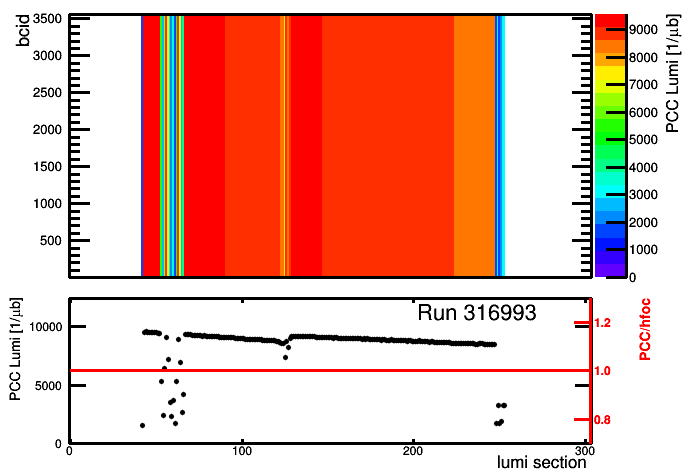
\includegraphics[width=0.52\columnwidth]{./316993.png}
  \caption{Top: Bunch crossing id (bcid) and PCC luminosity as a function of lumi section (1 lumi section is 23.36s). Bottom: PCC lumi as a function of lumi section using late run 2018D veto list for Run2018A.}
  \label{fig:CMS}
\end{figure}


\begin{figure}[H]
  \centering
  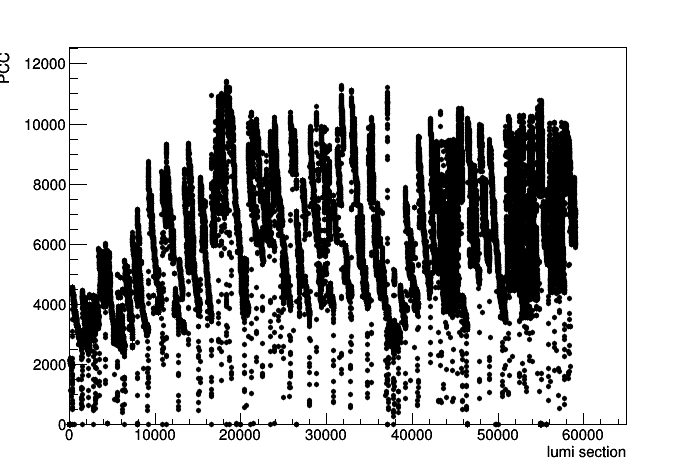
\includegraphics[width=0.52\columnwidth]{./ls_lumi.png}
  \caption{PCC luminosity ($\mu b^{-1}$) as a function of luminosity section (1 lumi section is 23.36s) for Run2018A.}
  \label{fig:CMS}
\end{figure}


\begin{figure}[H]
  \centering
  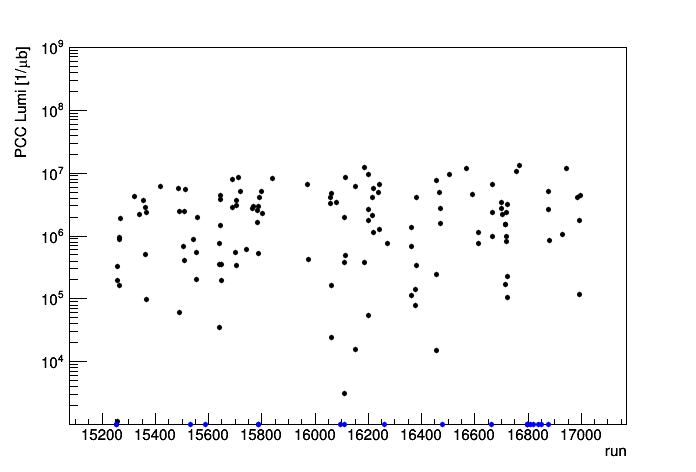
\includegraphics[width=0.52\columnwidth]{./runs.png}
  \caption{PCC luminosity ($\mu b^{-1}$) as a function of run number for Run2018A.}
  \label{fig:CMS}
\end{figure}


\begin{figure}[H]
  \centering
  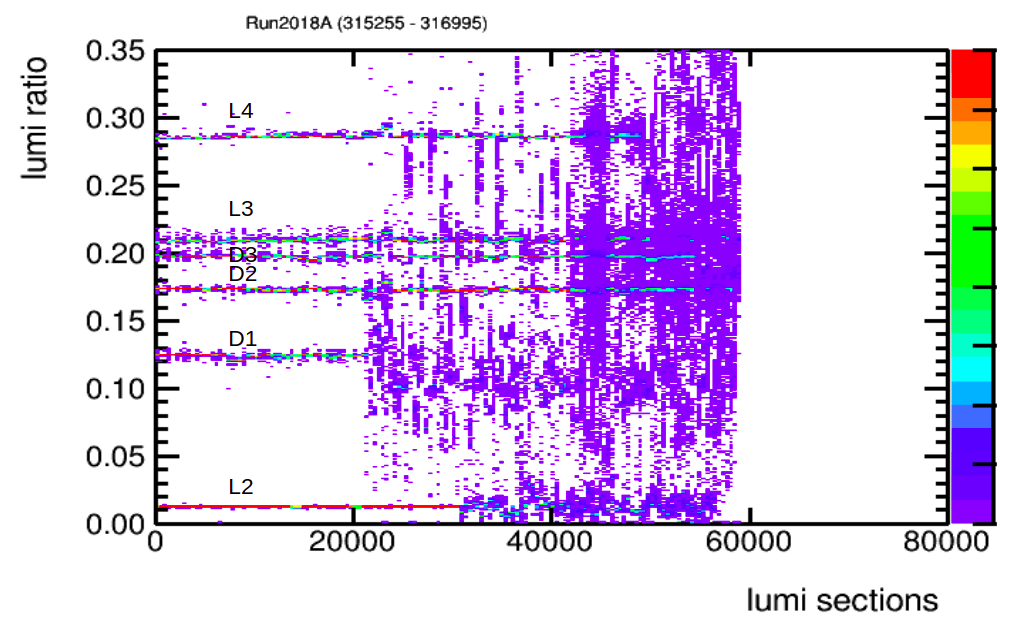
\includegraphics[width=0.52\columnwidth]{./2018A_lumiratio.png}
  \caption{Luminosity ratios for various subdetectors L2, L3, L4, D1, D2, D3 of pixel detector as a function of lumi section for Run2018A.}
  \label{fig:CMS}
\end{figure}



\begin{figure}[H]
  \centering
  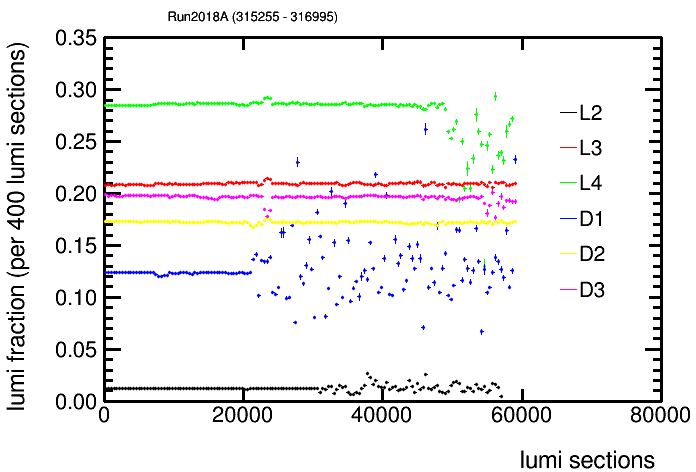
\includegraphics[width=0.52\columnwidth]{./ProfileXcombined_new.png}
  \caption{X Profile of luminosity ratios vs lumi section graph for various subdetectors L2, L3, L4, D1, D2, D3 of pixel detector showing luminosity fraction as a function of lumi section (1 lumi section is 23.36s) for Run2018A.}
  \label{fig:CMS}
\end{figure}





\begin{figure}[H]
  \centering
  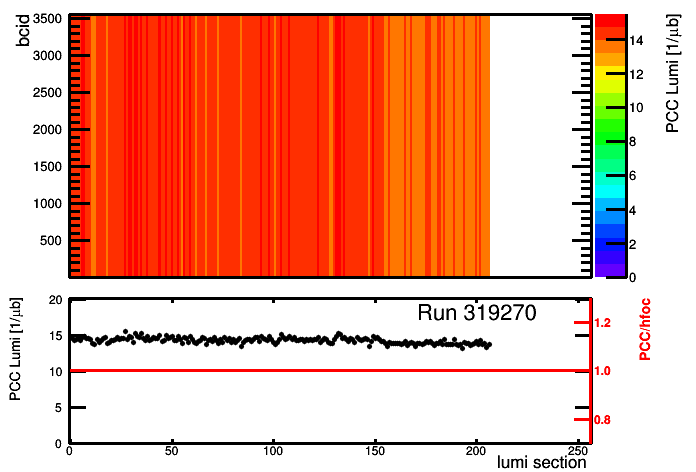
\includegraphics[width=0.52\columnwidth]{./319270.png}
  \caption{Top: Bunch crossing id (bcid) and PCC luminosity as a function of lumi section. Bottom: PCC lumi as a function of lumi section using late run 2018D veto list for Run2018B.}
  \label{fig:CMS}
\end{figure}


\begin{figure}[H]
  \centering
  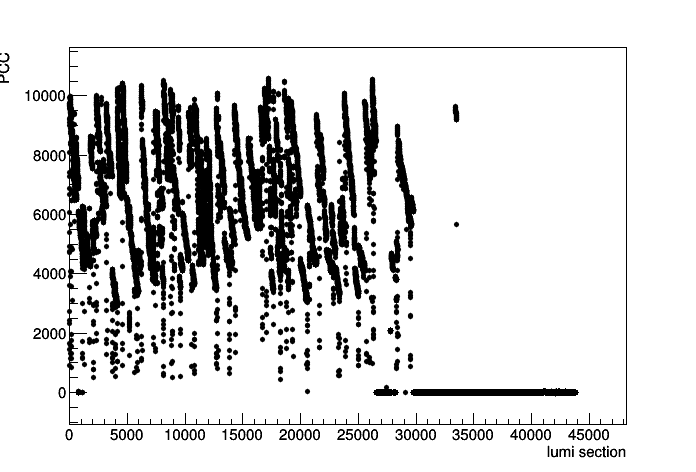
\includegraphics[width=0.52\columnwidth]{./ls_lumi_2018B.png}
  \caption{PCC luminosity as a function of lumi section for Run2018B.}
  \label{fig:CMS}
\end{figure}


\begin{figure}[H]
  \centering
  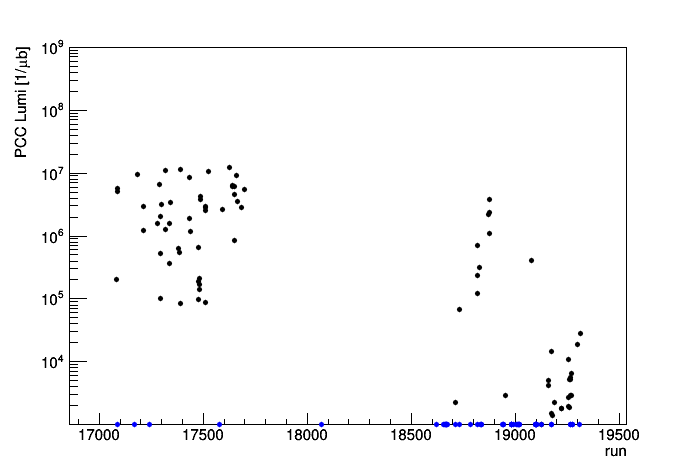
\includegraphics[width=0.52\columnwidth]{./runs_2018B.png}
  \caption{PCC luminosity as a function of run number for Run2018B.}
  \label{fig:CMS}
\end{figure}


\begin{figure}[H]
  \centering
  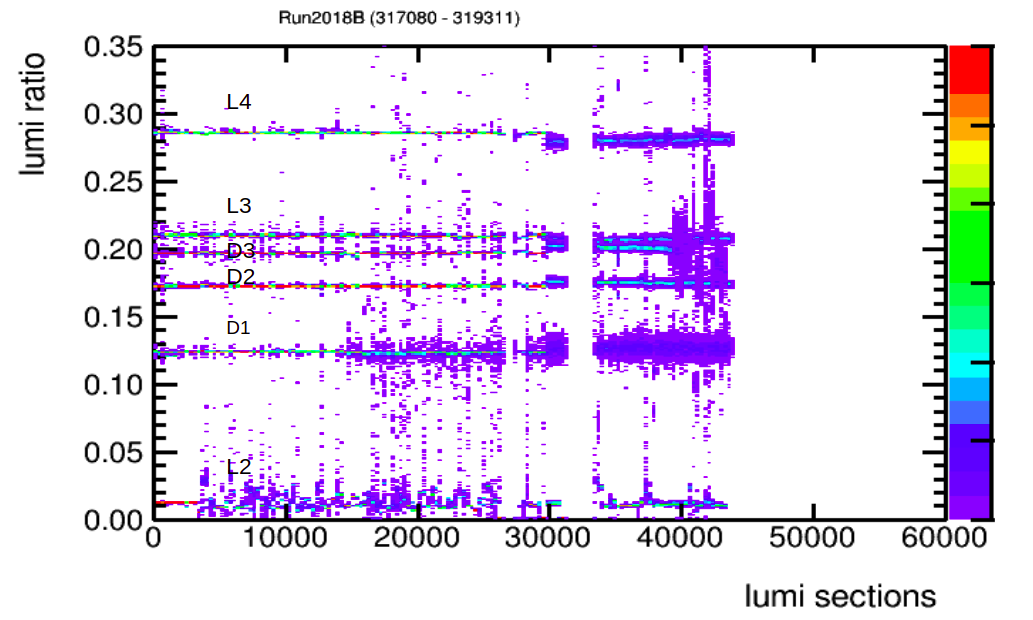
\includegraphics[width=0.52\columnwidth]{./2018B_lumiratio.png}
  \caption{Luminosity ratios for various subdetectors L2, L3, L4, D1, D2, D3 of pixel detector as a function of lumi section for Run2018B.}
  \label{fig:CMS}
\end{figure}



\begin{figure}[H]
  \centering
  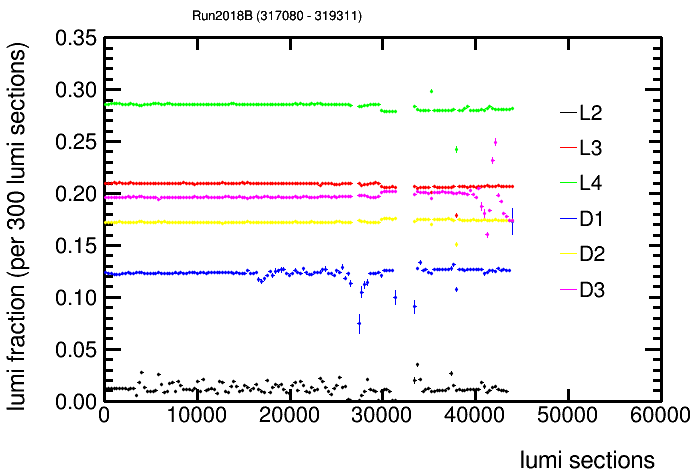
\includegraphics[width=0.5\columnwidth]{./ProfileXcombinedB_new.png}
  \caption{X Profile of luminosity ratios vs lumi section graph for various subdetectors L2, L3, L4, D1, D2, D3 of pixel detector showing luminosity fraction as a function of lumi section for Run2018B.}
  \label{fig:CMS}
\end{figure}



\begin{figure}[H]
  \centering
  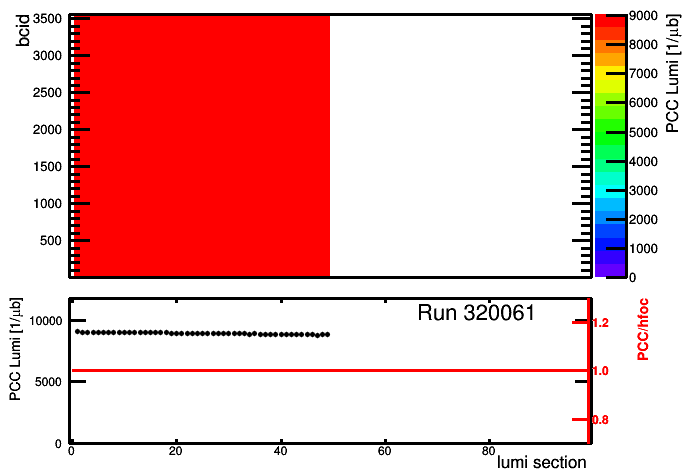
\includegraphics[width=0.5\columnwidth]{./320061.png}
  \caption{Top: Bunch crossing id (bcid) and PCC luminosity as a function of lumi section. Bottom: PCC lumi as a function of lumi section using late run 2018D veto list for Run2018C.}
  \label{fig:CMS}
\end{figure}


\begin{figure}[H]
  \centering
  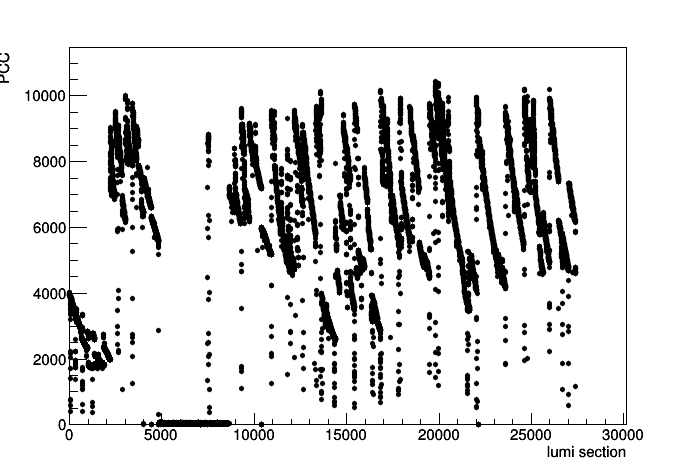
\includegraphics[width=0.5\columnwidth]{./ls_lumi_2018C.png}
  \caption{PCC luminosity as a function of lumi section for Run2018C.}
  \label{fig:CMS}
\end{figure}


\begin{figure}[H]
  \centering
  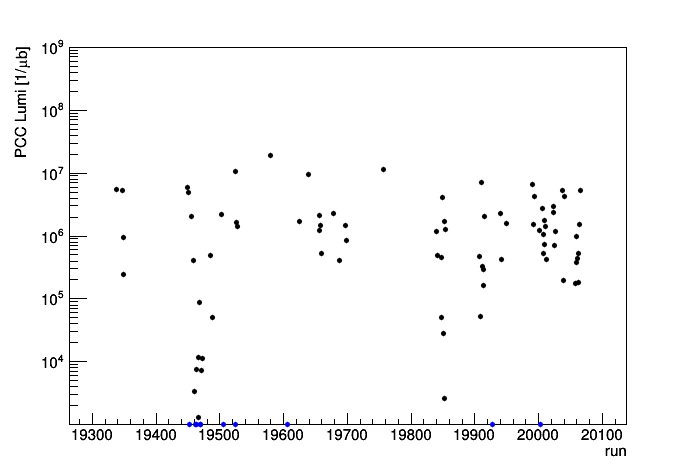
\includegraphics[width=0.5\columnwidth]{./runs_2018C.png}
  \caption{PCC luminosity as a function of run number for Run2018C.}
  \label{fig:CMS}
\end{figure}


\begin{figure}[H]
  \centering
  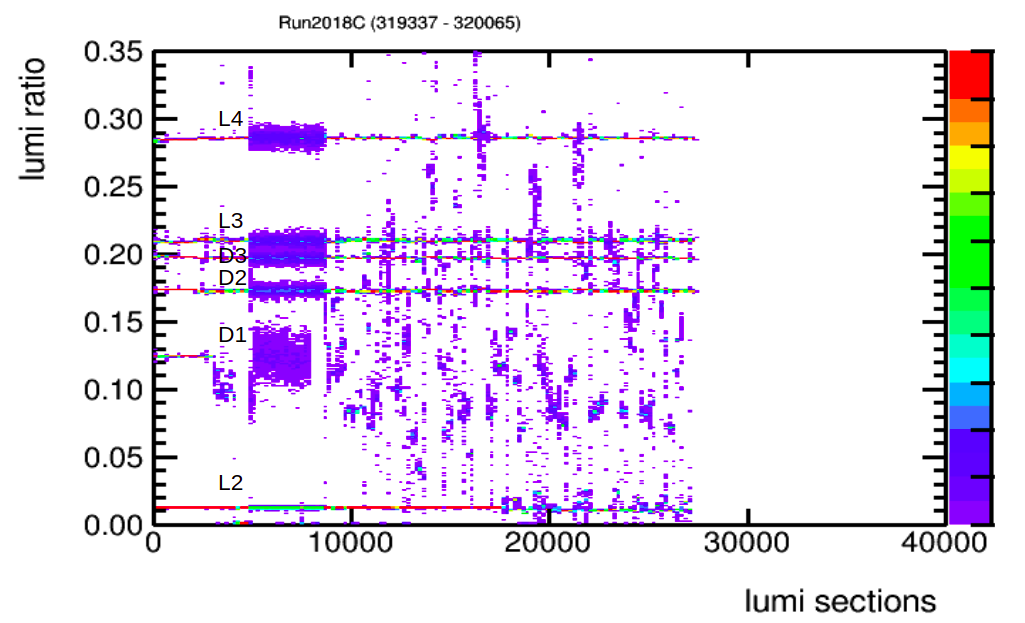
\includegraphics[width=0.5\columnwidth]{./2018C_lumiratio.png}
  \caption{Luminosity ratios for various subdetectors L2, L3, L4, D1, D2, D3 of pixel detector as a function of lumi section for Run2018C.}
  \label{fig:CMS}
\end{figure}


\begin{figure}[H]
  \centering
  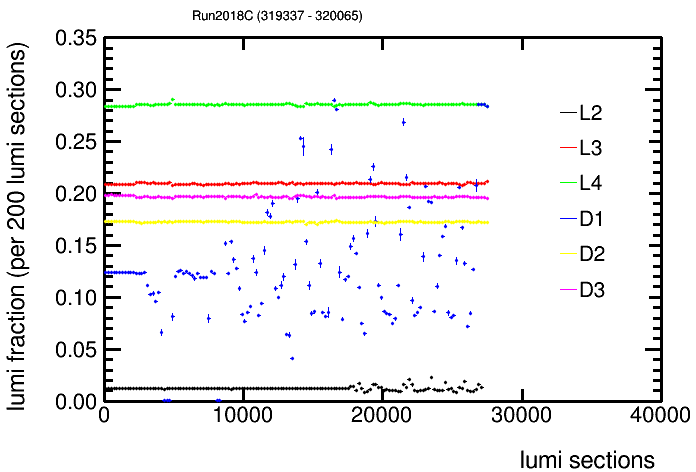
\includegraphics[width=0.5\columnwidth]{./ProfileXcombinedC_new.png}
  \caption{X Profile of luminosity ratios vs lumi section graph for various subdetectors L2, L3, L4, D1, D2, D3 of pixel detector showing luminosity fraction as a function of lumi section for Run2018C. \cite{lumidpg}}
  \label{fig:CMS}
\end{figure}


\end{verbatim}
%
then you could use the following commands
%
\vspace*{-2.5ex}\begin{verbatim}
  > tdr build myPaper   // build everything as a single PDF paper
  > tdr b results       // build just the results section as PDF
\end{verbatim}
%
In general you should be in the directory in which the
\LaTeX\ file resides. The script will search downwards in the directory tree for it, but if more than one version exists, it will not be able to determine which one to build. This situation (multiple copies of the top file) is guaranteed to occur once a tag or branch has been made, so it is important to note this.

%....................................
\subsection{Setting the default file to build}
%
To save specifying your preferred build target (\eg, \texttt{myPaper.tex}) each
time, just set the Unix environmental variable \texttt{TDR\_TARGET}
to \texttt{myPaper}.
Then you can just type
%
\vspace*{-2.5ex}\begin{verbatim}
  > tdr b
\end{verbatim}
%
If \texttt{TDR\_TARGET} has not been set, then \texttt{tdr} builds this document.

A similar variable, \texttt{TDR\_STYLE}, controls the default style.
%....................................
\subsection{Cleaning up}

To clean up temporary files (i.e the locally-created \texttt{tmp} directory):
\vspace*{-2.5ex}\begin{verbatim}
  > tdr clean
\end{verbatim}
%
To clean up temporary files and emacs and nedit backup files:
\vspace*{-2.5ex}\begin{verbatim}
  > tdr veryclean
\end{verbatim}



%----------------------------------------------------------------------------
\subsection{Formatting for journals\label{sec:journal-formatting}}
You can produce versions of your document formatted following the standards of several of the journals to which CMS submits physics results. Journal-specific options are passed as strings. To use
our defaults, use a single dash as the option:


\begin{verbatim}
tdr --style paper --aps - b XXX-08-000
\end{verbatim}

Please note that the \texttt{tdr} script can automatically take the pdfkeywords and format them for the equivalent journal field.

\begin{description}
\item[APS] use the normal command for a paper, but add the appropriate APS options with, \eg, \texttt{--aps="reprint,prl,linenumbers"}. See the revtex documentation for details on APS options. Information on the revtex style for use with APS journals can be found at \url{http://authors.aps.org/revtex4/} and download sites are listed at \url{https://authors.aps.org/revtex4/revtex4_faq.html#download}. APS does not accept sub-directories nor included \TeX files, so the necessary files will either be included or moved to the top level, as appropriate, for submission.
\item[PLB] use \texttt{--plb="3p,twocolumn,times"} or any other set of Elsevier options. See \url{http://www.elsevier.com/framework_authors/misc/elsdoc.pdf} for details on the Elsevier elsarticle style. As for the APS, PLB only accepts a flat file structure. The PLB default bib style will convert to lowercase all except the first word in the titles of references, so escape proper names, acronyms, \etc, with curly braces, \eg,\linebreak[4] "\verb|Search for {ADD} extra dimensional gravity|\ldots"
\item[EPJC] Please provide (using the if-then construction described below) a \verb|\titlerunning| in the text before the \verb|\maketitle|. This is used to create a running head so it cannot be longer than roughly half a page width. When EPJC sets articles, they tend to use the \verb|\sidecaption| macro and have caption plus two small plots run across the full page. This option is not accessible in the CMS style although one can pass it to the EPJC style via an if-then.
\item[JHEP] JHEP accepts papers in the CMS style.

\end{description}

For instances where the CMS style and the journal style are incompatible, one may use an \textit{if-then} construction to bracket alternatives:

\begin{verbatim}
\ifthenelse{\boolean{cms@external}}{%
%% journal specific text
}
{%
%CMS specific text
}
\end{verbatim}

Note, however, that many formatting changes that are required for the two-column format of many journals can be accommodated in the standard CMS style. Using the \texttt{*} format for figures that should extend across two columns does not effect placement for us. If you resize figures, use units of \verb|\columnwidth|, which is the same as the \verb|\textwidth| in single column format.
%----------------------------------------------------------------------------
\subsection{Supplemental material for journals\label{sec:journal-supplements}}
Supplemental material should be placed in an independent \LaTeX\ file, \eg, supplemental\_material.tex. This file will be included via conditional code in the main document (say GEN-12-001.tex, representing a GENeric document) when it is formatted for CMS and for the arXiv, and excluded in the journal version. A third file, GEN-12-001\_supp.tex should have the supplemental material included wrapped in a standard document template, which will provide an independent file for uploading to the journal.
So for GEN-12-001.tex,
\begin{verbatim}
...
\bibliography{auto_generated}
\ifthenelse{\boolean{cms@external}}{}{
\clearpage
\appendix
\numberwithin{table}{section}
\numberwithin{figure}{section}
\section{Supplemental information title\label{app:suppMat}}
\input{supplemental_material}
}
\end{verbatim}
while for GEN-12-001\_supp.tex,
\begin{verbatim}
\title{GEN-12-001 normal title \texorpdfstring{\\[1cm]
---Supplemental Material---}{: Supplemental Material}}
\author[cern]{The CMS Collaboration}
\date{\today}
\abstract{}
\hypersetup{%
...}
\maketitle
\null\cleardoublepage
\input{supplemental_material}
\end{verbatim}
The title of GEN-12-001 should be modified from that of the normal document: \verb|\title{|Normal Title\verb|\\[1cm]|---Supplemental Material---\verb|}|.
To generate all three types of files, arXiv (same as CMS format), PRL, and PRL supplement, the commands would be
\begin{verbatim}
tdr --style paper --aps - b GEN-12-001
tdr --style paper  b GEN-12-001
tdr --style paper --supplement --no-draft --preflight b GEN-12-001_supp
\end{verbatim}
You should specifically note how the supplemental material is referenced within the main file: the APS specifies, for instance, that the format for the reference in the text is ``See Supplemental Material at [URL will be inserted by publisher] for [give brief description of material]," so we use (for example) ``The results are available in tabulated form in \verb|\suppMaterial|", where we have defined \verb|\suppMaterial| in the GEN-12-001\_supp.tex file as
\begin{verbatim}
\ifthenelse{\boolean{cms@external}}
{\providecommand{\suppMaterial}{the supplemental material
  [URL will be inserted by publisher]}}
{\providecommand{\suppMaterial}{Appendix~\ref{app:suppMat}}}
\end{verbatim}
In the absence of a table of contents we can freely substitute anything we like for ``Appendix"  in the string above. If there is a table of contents, the \verb|\appendixname| should be conditionally redefined so that in CMS format it would be \verb|\renewcommand{\appendixname}{|Supplemental Material\verb|}|.


\clearpage
\section{Advice on using \texorpdfstring{\LaTeX}{LaTeX}\label{latex}}

%%%%%%%%%%%%%%%%%%%%%%%%%%%%%%%%%%%%%%%%%%%%%%%%%%%%%%%%%%%%%%%%%%%%
\subsection{\texorpdfstring{\LaTeX}{LaTeX} macros for commonly used constructs}

Provisions are made to implement macros across TDR volumes, within a
volume, or even locally in a particular section. However, in order to
establish a standard look and feel for the text symbols in the TDR
volumes
(such  as for $E_\text{T}$ and $p_\text{T}$),
we encourage use of the generally
defined macros and strongly discourage local use unless you are
certain a similar symbol would not be used by another editor.

At the top-most level, definitions defined in
{\texttt{tdr/utils/general/ptdr-definitions.sty}} are
available to all TDR volumes. An extensive set of macros have been
defined there and should be used whenever possible. They include, for
example, $\backslash$\texttt{ET}, $\backslash$\texttt{fbinv},
$\backslash$\texttt{sTop}, etc.
At the top-level of each TDR
(\eg, in \texttt{tdr/reports/ptdr1/tex/definitions.tex}, there is another
file \texttt{definitions.tex} for volume-specific definitions. Macros
should be suggested and implemented for
frequently used constructs or common symbols or names, \eg,
{$\backslash$\texttt{etc}}
could be defined to produce ``\emph{etc.}'' and so on.
The macros in the \texttt{definitions.tex} files are usable
in tex files at all levels of the particular TDR.

Use {$\backslash$\texttt{newcommand}} to define a new command that does not exist,
{$\backslash$\texttt{renewcommand}} to re-define a new command that already exists,
or {$\backslash$\texttt{providecommand}} to define a new command but accept the old
definition without complaint if it has already been defined.

To override a general definition in \texttt{TDR/general/ptdr-definitions.sty}
simply (re-)define it ( using \verb|\newcomand| or \verb|\renewcommand|) in the local \texttt{definitions.tex}. But please
consult with the appropriate TDR editor first.

We stress that it is important to use the macros in case a global style change must be made to suit the standards of a particular journal.

\subsection{Fonts}
Do not override the default fonts. They are currently set to be
Palatino and Helvetica. The math fonts have also been changed to
Palatino so that they do not clash with the body text,
particularly in regards to numbers and units. This means the
authors should use \verb|\text| commands to put text in subscripts
and superscripts, and most importantly \emph{do not use}
\verb|\rm| in formulas, otherwise you will end up with formulae looking like the second one below.

\begin{gather}
\phi = \text{a Greek letter}\\
{\rm \phi} = \text{a mistake}
\end{gather}

Also note that the math fonts include a full set of Greek symbols in Math Italic Bold (produced with \verb|\mathbold|),
but only uppercase in Math Bold (\verb|\mathbf|). Use \verb|\boldmath| or \verb|\boldsymbol| to get bold symbols: \verb|{\boldmath{$\alpha \otimes \beta$}}| : {\boldmath{$\alpha \otimes \beta$}}. (Note the enclosing braces.) Most journal styles do not have the \verb|\boldmath| command.



It is also advisable to use the \verb|\textrm{Some text}| form rather than
\verb|{\rm Some text}|. The same is true for the other short-form holdovers from plain \TeX,
\verb|\tt| and \verb|\it|, particularly if you would like to submit your paper to a journal
with minimal re-editing. For inclusion of text within an equation, \verb|\text| should be used.

%%%%%%%%%%%%%%%%%%%%%%%%%%%%%%%%%%%%%%%%%%%%%%%%%%%%%%%%%%%%%%%%%%%%
\subsection{Editorial macros}


In addition to the extensive measurement and physics symbols,
some editorial macros are defined in
\texttt{tdr/utils/general/definitions.tex} as well.
For example, the following tex fragment:
\begin{verbatim}
   \editor{Jane Doe} \\
   \contributor{Tom Cobbley} \\
   \fixme{check this number!} \\
\end{verbatim}
%
produces the following. \\
\bigbreak
\editor{Jane Doe}\mbox{~}\\
\contributor{Tom Cobbley}\mbox{~} \\
\fixme{check this number!}\mbox{~}\\

Notes use \texttt{author}, \texttt{address}, and \texttt{abstract} commands.



%%%%%%%%%%%%%%%%%%%%%%%%%%%%%%%%%%%%%%%%%%%%%%%%%%%%%%%%%%%%%%%%%%%%
\subsection{Inclusion of figures}

Figures should reside in the \texttt{fig} directory of the corresponding TDR (volume).
A figure may be included as follows:
%
%\vspace*{-2.5ex}
\begin{verbatim}
   Figure~\ref{fig:test} shows a figure prepared with the TDR
   template and illustrates how to include a picture in a document
   and refer to it using a symbolic label.
   \begin{figure}[!htb]
      \centering
      \includegraphics[width=0.55\textwidth]{c1_BlackAndWhite}
      \caption[Caption for TOC]{Test of graphics inclusion.\label{fig:test}}
   \end{figure}
\end{verbatim}
%
Please note that documents intended for journal submission should usually include the \texttt{fig} in the path name supplied to \texttt{includegraphics} and not rely on the automatic search.

The result of the above is roughly as follows:
%
% \clearpage

\begin{quote}
Figure~\ref{fig:test} shows a figure prepared with the TDR
    template and illustrates how to include
a picture in a document and refer to it using a symbolic label.
\end{quote}

    \begin{figure}[!htb]
      \centering
\vbox{
        \combinedfigure{width=0.55\textwidth}{c1}{c1}
      \caption[Caption for TOC]{Test of graphics inclusion.\label{fig:test}}
}
    \end{figure}

Note that the file extension (type) for the filename (\eg, \texttt{c1{\underline{\mbox{~}}}BlackAndWhite.pdf} above)
is not explicitly specified.
Also note that authors should use an alternate short caption within the
first set of brackets when the complete caption is unduly long for
including in the list of figures in the Table of Contents.

Also note that the current recommended size for figures is
\texttt{0.55$\backslash$textwidth} for square plots, and \texttt{0.7$\backslash$textwidth} for ones
with a standard (i.e., produced using the root template described in
Section~\ref{sec:root}) rectangular aspect ratio.

Finally, note that correct results for the labeling occur only if you
place the \texttt{label} command within the caption environment.


\subsubsection{Colour figures}

Figures will generally be printed in black and white for paper versions of the
final document.
We have found that the automatic conversion of colour figures to black and white
often results in a lack of legibility, so we recommend that all authors provide a
black and white version for each figure which they have checked for legibility
on an actual paper copy. If paper output is not required or the authors are satisfied with dual-purpose figures,
the rest of this section can be ignored.

Colour versions of figures can by provided for PDF output using the \verb+combinedfigure+ macro
in place of the  \texttt{$\backslash$includegraphics} command.
This takes two arguments corresponding  respectively to the black and white
and the coloured versions of the same picture, for example:
%
\vspace*{-2.5ex}\begin{verbatim}
   Figure~\ref{fig:test} shows a figure prepared with the TDR
   template and illustrates how to include a picture in a document
   and refer to it using a symbolic label.
   \begin{figure}[!htb]
      \centering
      \combinedfigure{width=0.4\textwidth}{c1_BlackAndWhite}{c1_Colour}
      \caption[Caption for TOC]{Test of graphics inclusion.\label{fig:test}}
   \end{figure}
\end{verbatim}
%
Both figures should have the same size or the pagination may be affected.


\subsubsection{How to include multiple figures}

If you need to include multiple figures into the figure environment
(i.e., you need only one common caption), the recommended procedure is to
use multiple instances of the \texttt{$\backslash$includegraphics} command, combined
with the \texttt{tabular} environment if needed. Please do not use the
\texttt{subfig} environment just to get ``(a)'' and ``(b)'' labels, it
is a waste of white space and does not look as nice as putting the
labels directly on the plot. Moreover, do not use the \texttt{picture}
environment to draw the labels, because the coordinate system is
absolute on the page and not relative to where the figure will be
placed (i.e., this only works for the very final version). In short, to
label multiple figures, it is best to embed the label into the plot.



%%%%%%%%%%%%%%%%%%%%%%%%%%%%%%%%%%%%%%%%%%%%%%%%%%%%%%%%%%%%%%%%%%%%
\subsubsection{How to handle figures in PDF, jpeg, and PS formats}

Files with extensions of \texttt{.pdf} (recommended) and \texttt{.jpg}
are automatically picked up.
Direct import of \texttt{.eps} files is not
supported by the \texttt{pdftex} driver which is used to convert
\LaTeX\ to PDF.
You are advised to convert your \texttt{.eps} file to a \texttt{.pdf} file
using Adobe Acrobat (best results), the \texttt{epstopdf}
command or \texttt{ps2pdf -dEPSCrop}, and commit that to \texttt{svn}.
Try to avoid converting figures through an intermediate program, such
as Powerpoint, and instead convert the natively produced
Postscript. If you do convert an EPS file, you are encouraged to also
commit the original EPS version as well in case of conversion
problems found later. The editors may re-convert if necessary.


%%%%%%%%%%%%%%%%%%%%%%%%%%%%%%%%%%%%%%%%%%%%%%%%%%%%%%%%%%%%%%%%%%%%
\subsubsection{Where to store figures}

In general the figures should reside in the \texttt{fig} directory or one
of its subdirectories.
A \texttt{fig} directory exists for each major document, \eg,
\texttt{tdr/reports/ptdr1/fig/} or \linebreak[3]\texttt{tdr/reports/ctdr/fig/}. Small papers with only a few figures do not
require the use of a subdirectory.

Do \emph{not} refer to any figures which reside outside the
TDR repository; instead, \texttt{svn add} the file in the \texttt{fig}
directory and check it in.

By default figures are looked for in the \texttt{fig} directory.

If a figure file resides in a subdirectory, \eg, \texttt{fig/muon},
of the \texttt{fig} directory, then simply prepend the directory
name when referring to the figure in the
\texttt{$\backslash${}includegraphics} command (i.e. \texttt{muon/c1} in the
above example).



%%%%%%%%%%%%%%%%%%%%%%%%%%%%%%%%%%%%%%%%%%%%%%%%%%%%%%%%%%%%%%%%%%%%
\subsubsection{Standard macro for figures produced with ROOT \label{sec:root}}

To maintain a standard look and feel for the figures in the Physics
TDRs, a Root macro was
contributed by Thomas Speer. Figure~\ref{fig:test} shows an example
plot made using it. In the TDR repository check out:
\texttt{tdr/utils/general/tdrstyle.C}. To use it:
%
\begin{verbatim}
.L tdrstyle.C
setTDRStyle()
\end{verbatim}

%%%%%%%%%%%%%%%%%%%%%%%%%%%%%%%%%%%%%%%%%%%%%%%%%%%%%%%%%%%%%%%%%%%%
\subsection{Convention for figure and table captions}

Figure captions should be located below each figure, as shown in the
example above. Table captions, however, should reside \emph{above}
the table and use \texttt{topcaption}.  For example:
%
\begin{verbatim}
\begin{table}[h]
  \begin{center}
    \topcaption{Table captions are above the table whereas figure
    captions are below.}
    \label{tab:mytab}
    \begin{tabular}{lcc} \hline
       Parameter & Value 1 & Value 2 \\ \hline
       $s$ & 10.0 & 20.0 \\
       $t$ & 20.0 & 30.0 \\
       $u$ & 30.0 & 40.0 \\ \hline
    \end{tabular}
  \end{center}
\end{table}
\end{verbatim}
%
which produces the following:
%
\begin{table}[h]
  \begin{center}
    \topcaption{Table captions are above the table whereas figure
    captions are below.}
    \label{tab:mytab}
    \begin{tabular}{lcc} \hline
       Parameter & Value 1 & Value 2 \\ \hline
       $s$ & 10.0 & 20.0 \\
       $t$ & 20.0 & 30.0 \\
       $u$ & 30.0 & 40.0 \\ \hline
    \end{tabular}
  \end{center}
\end{table}
%



%%%%%%%%%%%%%%%%%%%%%%%%%%%%%%%%%%%%%%%%%%%%%%%%%%%%%%%%%%%%%%%%%%%

\subsection{Chapters, sections and other sectioning commands}

For all notes use the following
section heading commands:
\texttt{$\backslash${}section},
\texttt{$\backslash${}subsection},
\texttt{$\backslash${}subsubsection}, and
\texttt{$\backslash${}paragraph}.
For Technical Design Reports the top-level sectioning command
is \texttt{$\backslash${}chapter} followed by all the above
sectioning commands.

The PDF bookmarks produced from Pdf\LaTeX\ will choke on \TeX symbols,
\eg, ``2.6 This is a
``026E30Fsection'' for ``2.6 This is a $\backslash$section'' since \TeX\ uses 026E30F to represent the backslash. Use the
\verb+\texorpdfstring+ macro:
\begin{verbatim}
\section{Finding the split \texorpdfstring{$A_2$}{A2}}
\end{verbatim}

And this is what it should look like:

\subsection{This is a \texorpdfstring{$\backslash$\texttt{subsection}}{subsection}}
This is some text.

\subsubsection{This is a \texorpdfstring{$\backslash$\texttt{subsubsection}}{subsubsection}}
This is some text.


\paragraph{This is a \texorpdfstring{$\backslash$\texttt{paragraph}}{paragraph}}
This is some text.




%%%%%%%%%%%%%%%%%%%%%%%%%%%%%%%%%%%%%%%%%%%%%%%%%%%%%%%%%%%%%%%%%%%%

\subsection{Cross-references and bibliographic citations}

\subsubsection{Referring to Sections, Figures, Tables, etc.}
\texorpdfstring{\LaTeX}{LaTeX} provides powerful, robust, and scalable facilities for
cross-referencing based on symbolic labels.
Please use them!

For example, to create symbolic links to a chapter
and a section:
%
\vspace*{-2.5ex}\begin{verbatim}
   \chapter{Mass Storage Systems\label{ch:mss}}
   \section{Requirements\label{sec:mss-requirements}}
\end{verbatim}
%
Note that the \texttt{label} command is contained \emph{within} the
curly braces of the appropriate sectioning command so that
the value can be resolved correctly.
For figures and tables, the \texttt{label} command should be
similarly enclosed within the associated \texttt{caption} command.

To then refer to the chapter and section:
\vspace*{-2.5ex}\begin{verbatim}
   The CMS hierarchical mass storage systems, described in
   Chapter~\ref{ch:mss} will be of a size unprecedented in
   HEP, as described in Section~\ref{sec:mss-requirements}.
\end{verbatim}

This will result in output something like:
\begin{quote}
   The CMS hierarchical mass storage systems, described in
   Chapter~9 will be of a size unprecedented in
   HEP, as described in Section~9.1.
\end{quote}
%
Note that the numbers (9 and 9.1) are automatically generated
according to the placement of the \texttt{label} commands
in the overall context of the document.
The number of digits (levels) is determined automatically from
the level of the sectioning command used (chapter, section,
subsection, etc.).

Always -- \emph{repeat always} -- use symbolic labels
(\eg, \texttt{sec:mss-requirements})
for references and not hardwired numbers
(\eg, \texttt{9.1})
as the latter will invariably become wrong very quickly.



%%%%%%%%%%%%%%%%%%%%%%%%%%%%%%%%%%%%%%%%%%%%%%%%%%%%%%%%%%%%%%%%%%%%

\subsubsection{Bibliographic references}

All bibliographic entries are defined in a BibTeX file
(i.e., files with \texttt{.bib} extension in the \texttt{bib} directory
of the TDR (volume) of interest.
This enables a standard format to be ensured and helps avoid
duplicated entries.
Before defining a new bibliographic item, please check in the
\texttt{.bib} files whether it has already been defined, and if so
then use it as it is. When creating new BibTeX entries, the format of
the bibliographic entries is mostly self-evident and one can
cut-and-paste from an existing entry (well, check that it produces
reasonable output) and then change the text.

Keep in mind that for listing authors, the BibTeX implementation uses
``Last Name, First Name'' (and it automatically abbreviates the first
name). Concatenate authors using ``and'', and instead of writing
``\emph{et al.}'' use ``and others.'' BibTeX will handle the substitution,
and our style file will trim the author list automatically after three authors. For
complicated names, you can place them in braces ${}$, but do this
sparingly.


We strongly recommend the use of the \href{http://inspirehep.net}{inSPIRE} BibTeX labels when such an
article can be found there, because a unique label is created and
\LaTeX\ can spot multiply-defined references. It also saves you the time
of creating the entry yourself. Such an entry looks like:

\begin{verbatim}
@Article{Agostinelli:2002hh,
     author    = "Agostinelli, S. and others",
     collaboration = "GEANT4",
     title     = "{GEANT4}---a simulation toolkit",
     journal   = nim,
     volume    = "A506",
     year      = "2003",
     pages     = "250-303",
     SLACcitation  = "%%CITATION = NUIMA,A506,250;%%",
     DOI       = "10.1016/S0168-9002(03)01368-8"
}
\end{verbatim}

However, in the above instance and for many other \emph{commonly} cited
references, we will use a more conventional name (\eg,
GEANT4 instead of Agostinelli:2002hh). So please check the other bibliography files to see if yours
is already defined. The information should also be verified. In the above citation, the title was not quite right on inSPIRE.

In addition, we recommend setting the ``DOI'' field that was added to
the Article BibTeX format in the TDR framework (and is illustrated
above). This field represents
the Digital Object
Identifier for your reference.\footnote{\url{http://www.doi.org/}}
When you prepend this number with \url{http://dx.doi.org/}, your
browser is automatically directed to the electronic version of the
article (provided your institution has paid for this access). Currently
you need to manually determine and enter this field after examining the
publication.

To refer to an item in the bibliography using its symbolic label
in your text, use one of the following forms:
\vspace*{-2.5ex}\begin{verbatim}
   Either: the CMS detector is described elsewhere~\cite{CMSTP};
   or: the CMS detector is described in reference~\citenum{CMSTP}.
\end{verbatim}

This will result in output something like:
\begin{quote}
   Either: the CMS detector is described elsewhere~[34];
   or: the CMS detector is described in reference~34.
\end{quote}
%
Note the omission of the square brackets in the second form,
where the reference is explicitly (rather than parenthetically)
referred to.

The list of references will be placed at the end of the TDR. It is
suggested that each group maintain a separate \texttt{.bib} file in the
\texttt{bib} directory for the chapter specific references. Common
references for the entire TDR will be kept in a common file (\eg, ptdr1.bib). Common software references will be kept in
software.bib.

\subsubsection{Web References}
Please use the \verb+\href+ and \verb+\url+ commands to embed links into your document (these are not allowed in journal submissions).

Example:\\
\verb+\url{http://cms.cern.ch/iCMS/}+ gives \url{http://cms.cern.ch/iCMS/},\\
\verb+\href{http://cms.cern.ch/iCMS/}{The CMS web site}+ gives \href{http://cms.cern.ch/iCMS/}{The CMS web site}.

%%%%%%%%%%%%%%%%%%%%%%%%%%%%%%%%%%%%%%%%%%%%%%%%%%%%%%%%%%%%%%%%%%%%

% \clearpage
\subsection{Glossary}

Please add a short entry to \texttt{glossary.tex}
whenever introducing any new acronym or abbreviation.
Even plain English terms with specific technical
meaning should be included (\eg, Python).
\setlength{\columnseprule}{0.2mm}
\setlength{\multicolsep}{7mm}
\providecommand{\symexamp}[2]
{
\makebox[0.160\textwidth][l]{#1:}
                          \makebox[0.025\textwidth][l]{~}
                          \parbox[t]{0.32\textwidth}{#2\vspace*{-2.5mm}\\}}

\clearpage
\section{PTDR Symbol Definitions}
%
\begin{multicols}{2}
%
\small%
\raggedcolumns%

\symexamp{etal}{\etal}
\symexamp{ie}{\ie}
\symexamp{eg}{\eg}
\symexamp{etc}{\etc}
\symexamp{vs}{\vs}
\symexamp{mdash}{\mdash}
\symexamp{NA}{\NA}
\symexamp{Lone}{\Lone}
\symexamp{Ltwo}{\Ltwo}
\symexamp{Lthree}{\Lthree}
\symexamp{ACERMC}{\ACERMC}
\symexamp{ALPGEN}{\ALPGEN}
\symexamp{BLACKHAT}{\BLACKHAT}
\symexamp{CALCHEP}{\CALCHEP}
\symexamp{CHARYBDIS}{\CHARYBDIS}
\symexamp{CMKIN}{\CMKIN}
\symexamp{CMSIM}{\CMSIM}
\symexamp{CMSSW}{\CMSSW}
\symexamp{COBRA}{\COBRA}
\symexamp{COCOA}{\COCOA}
\symexamp{COMPHEP}{\COMPHEP}
\symexamp{EVTGEN}{\EVTGEN}
\symexamp{FAMOS}{\FAMOS}
\symexamp{FASTJET}{\FASTJET}
\symexamp{FEWZ}{\FEWZ}
\symexamp{GARCON}{\GARCON}
\symexamp{GARFIELD}{\GARFIELD}
\symexamp{GEANE}{\GEANE}
\symexamp{GEANTfour}{\GEANTfour}
\symexamp{GEANTthree}{\GEANTthree}
\symexamp{GEANT}{\GEANT}
\symexamp{HDECAY}{\HDECAY}
\symexamp{HERWIG}{\HERWIG}
\symexamp{HERWIGpp}{\HERWIGpp}
\symexamp{POWHEG}{\POWHEG}
\symexamp{HIGLU}{\HIGLU}
\symexamp{HIJING}{\HIJING}
\symexamp{HYDJET}{\HYDJET}
\symexamp{IGUANA}{\IGUANA}
\symexamp{ISAJET}{\ISAJET}
\symexamp{ISAPYTHIA}{\ISAPYTHIA}
\symexamp{ISASUGRA}{\ISASUGRA}
\symexamp{ISASUSY}{\ISASUSY}
\symexamp{ISAWIG}{\ISAWIG}
\symexamp{MADGRAPH}{\MADGRAPH}
\symexamp{MCATNLO}{\MCATNLO}
\symexamp{MCFM}{\MCFM}
\symexamp{MILLEPEDE}{\MILLEPEDE}
\symexamp{ORCA}{\ORCA}
\symexamp{OSCAR}{\OSCAR}
\symexamp{PHOTOS}{\PHOTOS}
\symexamp{PROSPINO}{\PROSPINO}
\symexamp{PYTHIA}{\PYTHIA}
\symexamp{SHERPA}{\SHERPA}
\symexamp{TAUOLA}{\TAUOLA}
\symexamp{TOPREX}{\TOPREX}
\symexamp{XDAQ}{\XDAQ}
\symexamp{MGvATNLO}{\MGvATNLO}
\symexamp{DZERO}{\DZERO}
\symexamp{de}{\de}
\symexamp{ten\{x\}}{\ten{x}}
\symexamp{unit\{x\}}{\unit{x}}
\symexamp{mum}{\mum {\tiny[Most units include leading thinspace]}}
\symexamp{micron}{\micron}
\symexamp{cm}{\cm}
\symexamp{mm}{\mm}
\symexamp{mus}{\mus}
\symexamp{keV}{\keV}
\symexamp{MeV}{\MeV}
\symexamp{MeVns}{\MeVns\hspace{\fill}{\tiny[\textit{no} leading thinspace with \textit{ns} suffix]}}
\symexamp{GeV}{\GeV}
\symexamp{GeVns}{\GeVns}
\symexamp{gev}{\gev}
\symexamp{TeV}{\TeV}
\symexamp{TeVns}{\TeVns}
\symexamp{PeV}{\PeV}
\symexamp{keVc}{\keVc}
\symexamp{MeVc}{\MeVc}
\symexamp{GeVc}{\GeVc}
\symexamp{GeVcns}{\GeVcns}
\symexamp{TeVc}{\TeVc}
\symexamp{keVcc}{\keVcc}
\symexamp{MeVcc}{\MeVcc}
\symexamp{GeVcc}{\GeVcc}
\symexamp{GeVccns}{\GeVccns}
\symexamp{TeVcc}{\TeVcc}
\symexamp{pbinv}{\pbinv}
\symexamp{fbinv}{\fbinv}
\symexamp{nbinv}{\nbinv}
\symexamp{mubinv}{\mubinv}
\symexamp{mbinv}{\mbinv}
\symexamp{percms}{\percms}
\symexamp{lumi}{\lumi}
\symexamp{Lumi}{\Lumi}
\symexamp{LvLow}{\LvLow}
\symexamp{LLow}{\LLow}
\symexamp{lowlumi}{\lowlumi}
\symexamp{LMed}{\LMed}
\symexamp{LHigh}{\LHigh}
\symexamp{hilumi}{\hilumi}
\symexamp{PT}{\PT}
\symexamp{pt}{\pt}
\symexamp{ET}{\ET}
\symexamp{HT}{\HT}
\symexamp{mT}{\mT}
\symexamp{mTii}{\mTii}
\symexamp{et}{\et}
\symexamp{Em}{\Em}
\symexamp{Pm}{\Pm}
\symexamp{PTm}{\PTm}
\symexamp{PTslash}{\PTslash}
\symexamp{ETm}{\ETm}
\symexamp{MET}{\MET}
\symexamp{ETmiss}{\ETmiss}
\symexamp{ptmiss}{\ptmiss}
\symexamp{ETslash}{\ETslash}
\symexamp{VEtmiss}{\VEtmiss}
\symexamp{ptvec}{\ptvec}
\symexamp{ptvecmiss}{\ptvecmiss}
\symexamp{tauh}{\tauh}
\symexamp{sqrtsNN}{\sqrtsNN}
\symexamp{mht}{\mht}
\symexamp{htvecmiss}{\htvecmiss}
\symexamp{dd\{y\}\{x\}}{\dd{y}{x}}
\symexamp{ddinline\{y\}\{x\}}{\ddinline{y}{x}}
\symexamp{rd}{\rd}
\symexamp{re}{\re}
\symexamp{abs\{x\}}{\abs{x}}
\symexamp{CL}{\CL}
\symexamp{CLs}{\CLs}
\symexamp{CLsb}{\CLsb}
\symexamp{zp}{\zp}
\symexamp{JPsi}{\JPsi}
\symexamp{Z}{\Z}
\symexamp{ttbar}{\ttbar}
\noindent%
\textcolor{gray}{\rule{\columnwidth}{0.2pt}}
\noindent%
\textcolor{gray}{\rule{\columnwidth}{0.2pt}}
\noindent%
\textcolor{gray}{\rule{\columnwidth}{0.2pt}}\\
\noindent%
Other\\
\symexamp{AFB}{\AFB}
\symexamp{wangle}{\wangle}
\symexamp{stat}{\stat\hspace{\fill}{\tiny[Includes leading thinspace]}}
\symexamp{syst}{\syst\hspace{\fill}{\tiny[Includes leading thinspace]}}
\symexamp{thy}{\thy\hspace{\fill}{\tiny[Includes leading thinspace]}}
\symexamp{lum}{\lum\hspace{\fill}{\tiny[Includes leading thinspace]}}
\symexamp{kt}{\kt}
\symexamp{BC}{\BC}
\symexamp{bbarc}{\bbarc}
\symexamp{bbbar}{\bbbar}
\symexamp{ccbar}{\ccbar}
\symexamp{qqbar}{\qqbar}
\symexamp{MD}{\MD}
\symexamp{Mpl}{\Mpl}
\symexamp{Rinv}{\Rinv}
\noindent%
\textcolor{gray}{\rule{\columnwidth}{0.2pt}}\\
\noindent%
Older definitions (may be deprecated)\hspace{\fill}
\symexamp{bspsiphi}{\bspsiphi}
\symexamp{EE}{\EE}
\symexamp{MM}{\MM}
\symexamp{TT}{\TT}
\symexamp{HGG}{\HGG}
\symexamp{GAMJET}{\GAMJET}
\symexamp{PPTOJETS}{\PPTOJETS}
\symexamp{PPTOGG}{\PPTOGG}
\symexamp{PPTOGAMJET}{\PPTOGAMJET}
\symexamp{MH}{\MH}
\symexamp{RNINE}{\RNINE}
\symexamp{DR}{\DR}
\symexamp{ga}{\ga}
\symexamp{la}{\la}
\symexamp{swsq}{\swsq}
\symexamp{cwsq}{\cwsq}
\symexamp{tanb}{\tanb}
\symexamp{tanbsq}{\tanbsq}
\symexamp{sidb}{\sidb}
\symexamp{alpS}{\alpS}
\symexamp{alpt}{\alpt}
\symexamp{QL}{\QL}
\symexamp{sQ}{\sQ}
\symexamp{sQL}{\sQL}
\symexamp{ULC}{\ULC}
\symexamp{sUC}{\sUC}
\symexamp{sULC}{\sULC}
\symexamp{DLC}{\DLC}
\symexamp{sDC}{\sDC}
\symexamp{sDLC}{\sDLC}
\symexamp{LL}{\LL}
\symexamp{sL}{\sL}
\symexamp{sLL}{\sLL}
\symexamp{ELC}{\ELC}
\symexamp{sEC}{\sEC}
\symexamp{sELC}{\sELC}
\symexamp{sEL}{\sEL}
\symexamp{sER}{\sER}
\symexamp{sFer}{\sFer}
\symexamp{sQua}{\sQua}
\symexamp{sUp}{\sUp}
\symexamp{suL}{\suL}
\symexamp{suR}{\suR}
\symexamp{sDw}{\sDw}
\symexamp{sdL}{\sdL}
\symexamp{sdR}{\sdR}
\symexamp{sTop}{\sTop}
\symexamp{stL}{\stL}
\symexamp{stR}{\stR}
\symexamp{stone}{\stone}
\symexamp{sttwo}{\sttwo}
\symexamp{sBot}{\sBot}
\symexamp{sbL}{\sbL}
\symexamp{sbR}{\sbR}
\symexamp{sbone}{\sbone}
\symexamp{sbtwo}{\sbtwo}
\symexamp{sLep}{\sLep}
\symexamp{sLepC}{\sLepC}
\symexamp{sEl}{\sEl}
\symexamp{sElC}{\sElC}
\symexamp{seL}{\seL}
\symexamp{seR}{\seR}
\symexamp{snL}{\snL}
\symexamp{sMu}{\sMu}
\symexamp{sNu}{\sNu}
\symexamp{sTau}{\sTau}
\symexamp{Glu}{\Glu}
\symexamp{sGlu}{\sGlu}
\symexamp{Wpm}{\Wpm}
\symexamp{sWpm}{\sWpm}
\symexamp{Wz}{\Wz}
\symexamp{sWz}{\sWz}
\symexamp{sWino}{\sWino}
\symexamp{Bz}{\Bz}
\symexamp{sBz}{\sBz}
\symexamp{sBino}{\sBino}
\symexamp{Zz}{\Zz}
\symexamp{sZino}{\sZino}
\symexamp{sGam}{\sGam}
\symexamp{chiz}{\chiz}
\symexamp{chip}{\chip}
\symexamp{chim}{\chim}
\symexamp{chipm}{\chipm}
\symexamp{Hone}{\Hone}
\symexamp{sHone}{\sHone}
\symexamp{Htwo}{\Htwo}
\symexamp{sHtwo}{\sHtwo}
\symexamp{sHig}{\sHig}
\symexamp{sHa}{\sHa}
\symexamp{sHb}{\sHb}
\symexamp{sHpm}{\sHpm}
\symexamp{hz}{\hz}
\symexamp{Hz}{\Hz}
\symexamp{Az}{\Az}
\symexamp{Hpm}{\Hpm}
\symexamp{sGra}{\sGra}
\symexamp{mtil}{\mtil}
\symexamp{rpv}{\rpv}
\symexamp{LLE}{\LLE}
\symexamp{LQD}{\LQD}
\symexamp{UDD}{\UDD}
\symexamp{Lam}{\Lam}
\symexamp{Lamp}{\Lamp}
\symexamp{Lampp}{\Lampp}
\end{multicols}
\clearpage
\section{Particle symbols: PENNAMES2 \label{pennames}}
\ifthenelse{\boolean{cms@external}}{}{\vspace*{-5mm}
\begin{multicols}{2}
%
\raggedcolumns%
}
%
\newcommand{\head}[1]{\leavevmode\textcolor{gray}{\leaders\hbox{\rule[0.3em]{1pt}{0.1ex}}\hfill\kern0pt#1\leaders\hbox{\rule[0.3em]{1pt}{0.1ex}}\hfill\kern0pt}\\} %https://stackoverflow.com/questions/2553392/latex-rule-filling-the-line
\head{ Standard model bosons and Higgs}
\symexamp{Pg}{\Pg}
\symexamp{PGg}{\PGg}
\symexamp{PW}{\PW}
\symexamp{PWpm}{\PWpm}
\symexamp{PWmp}{\PWmp}
\symexamp{PWp}{\PWp}
\symexamp{PWm}{\PWm}
\symexamp{PZ}{\PZ}
\symexamp{PZz}{\PZz}
\symexamp{PH}{\PH}
\symexamp{PHz}{\PHz}
\symexamp{PWDt}{\PWDt}
\head{W and Z Bosons outside Standard Model}
\symexamp{PWpDt}{\PWpDt}
\symexamp{PWpr}{\PWpr}
\symexamp{PWL}{\PWL}
\symexamp{PWR}{\PWR}
\symexamp{PZpr}{\PZpr}
\symexamp{PZprpr}{\PZprpr}
\symexamp{PZst}{\PZst}
\symexamp{PZzDt}{\PZzDt}
\symexamp{PZzDT}{\PZzDT}
\symexamp{PZL}{\PZL}
\symexamp{PZLR}{\PZLR}
\symexamp{PZR}{\PZR}
\symexamp{PZGc}{\PZGc}
\symexamp{PZGe}{\PZGe}
\symexamp{PZGy}{\PZGy}
\head{LEPTONS}
\symexamp{Pl}{\Pl}
\symexamp{PlR}{\PlR}
\symexamp{Plpm}{\Plpm}
\symexamp{Plp}{\Plp}
\symexamp{Plm}{\Plm}
\symexamp{PlmR}{\PlmR}
\symexamp{PAl}{\PAl}
\symexamp{PGnl}{\PGnl}
\symexamp{PAGnl}{\PAGnl}
\symexamp{Pe}{\Pe}
\symexamp{Pepm}{\Pepm}
\symexamp{Pemp}{\Pemp}
\symexamp{Pem}{\Pem}
\symexamp{Pep}{\Pep}
\symexamp{PGb}{\PGb}
\symexamp{PGbm}{\PGbm}
\symexamp{PGbp}{\PGbp}
\symexamp{PGm}{\PGm}
\symexamp{PGmpm}{\PGmpm}
\symexamp{PGmm}{\PGmm}
\symexamp{PGmp}{\PGmp}
\symexamp{PGt}{\PGt}
\symexamp{PGtpm}{\PGtpm}
\symexamp{PGtm}{\PGtm}
\symexamp{PGtp}{\PGtp}
\symexamp{PGtpr}{\PGtpr}
\symexamp{PGtprm}{\PGtprm}
\symexamp{PGtprp}{\PGtprp}
\symexamp{PGn}{\PGn}
\symexamp{PGne}{\PGne}
\symexamp{PGnGm}{\PGnGm}
\symexamp{PGnGt}{\PGnGt}
\symexamp{PGnGtpr}{\PGnGtpr}
\symexamp{PAGn}{\PAGn}
\symexamp{PAGne}{\PAGne}
\symexamp{PAGnGm}{\PAGnGm}
\symexamp{PAGnGt}{\PAGnGt}
\symexamp{PAGnGtpr}{\PAGnGtpr}
\symexamp{PL}{\PL}
\symexamp{PLm}{\PLm}
\symexamp{PLp}{\PLp}
\symexamp{PLz}{\PLz}
\symexamp{PLpm}{\PLpm}
\symexamp{PAL}{\PAL}
\head{ QUARKS }
\symexamp{PQq}{\PQq}
\symexamp{PQd}{\PQd}
\symexamp{PQu}{\PQu}
\symexamp{PQs}{\PQs}
\symexamp{PQc}{\PQc}
\symexamp{PQb}{\PQb}
\symexamp{PQt}{\PQt}
\symexamp{PQbpr}{\PQbpr}
\symexamp{PQtpr}{\PQtpr}
\symexamp{PAQq}{\PAQq}
\symexamp{PAQd}{\PAQd}
\symexamp{PAQu}{\PAQu}
\symexamp{PAQs}{\PAQs}
\symexamp{PAQc}{\PAQc}
\symexamp{PAQb}{\PAQb}
\symexamp{PAQt}{\PAQt}
\symexamp{PAQbpr}{\PAQbpr}
\symexamp{PAQtpr}{\PAQtpr}
\symexamp{PQqb}{\PQqb}
\symexamp{PQqbpr}{\PQqbpr}
\symexamp{PQqc}{\PQqc}
\symexamp{PQqd}{\PQqd}
\symexamp{PQqdR}{\PQqdR}
\symexamp{PQqs}{\PQqs}
\symexamp{PQqt}{\PQqt}
\symexamp{PQqtpr}{\PQqtpr}
\symexamp{PQqu}{\PQqu}
\symexamp{PQquR}{\PQquR}
\symexamp{PAQqb}{\PAQqb}
\symexamp{PAQqbpr}{\PAQqbpr}
\symexamp{PAQqc}{\PAQqc}
\symexamp{PAQqd}{\PAQqd}
\symexamp{PAQqs}{\PAQqs}
\symexamp{PAQqt}{\PAQqt}
\symexamp{PAQqtpr}{\PAQqtpr}
\symexamp{PAQqu}{\PAQqu}
\head{ BARYONS  }
\symexamp{Pp}{\Pp}
\symexamp{Pn}{\Pn}
\symexamp{PAp}{\PAp}
\symexamp{PAn}{\PAn}
\symexamp{PGa}{\PGa}
\symexamp{PN}{\PN}
\symexamp{PNp}{\PNp}
\symexamp{PNz}{\PNz}
\symexamp{PNP\{x\}}{\PNP{x}}
\symexamp{PNpP\{x\}}{\PNpP{x}}
\symexamp{PNzP\{x\}}{\PNzP{x}}
\symexamp{PGD}{\PGD}
\symexamp{PGDpp}{\PGDpp}
\symexamp{PGDp}{\PGDp}
\symexamp{PGDz}{\PGDz}
\symexamp{PGDm}{\PGDm}
\symexamp{PGDP\{x\}}{\PGDP{x}}
\symexamp{PGDppP\{x\}}{\PGDppP{x}}
\symexamp{PGDpP\{x\}}{\PGDpP{x}}
\symexamp{PGDzP\{x\}}{\PGDzP{x}}
\symexamp{PGDmP\{x\}}{\PGDmP{x}}
\symexamp{PGQpP\{x\}}{\PGQpP{x}}
\symexamp{PGFP\{x\}}{\PGFP{x}}
\symexamp{PGL}{\PGL}
\symexamp{PAGL}{\PAGL}
\symexamp{PGLP\{x\}}{\PGLP{x}}
\symexamp{PGLc}{\PGLc}
\symexamp{PGLpc}{\PGLpc}
\symexamp{PGLpcP\{x\}}{\PGLpcP{x}}
\symexamp{PGLb}{\PGLb}
\symexamp{PGLzb}{\PGLzb}
\symexamp{PGS}{\PGS}
\symexamp{PAGS}{\PAGS}
\symexamp{PGSpm}{\PGSpm}
\symexamp{PGSm}{\PGSm}
\symexamp{PGSp}{\PGSp}
\symexamp{PGSz}{\PGSz}
\symexamp{PGSstm}{\PGSstm}
\symexamp{PGSstp}{\PGSstp}
\symexamp{PGSstz}{\PGSstz}
\symexamp{PGSP\{x\}}{\PGSP{x}}
\symexamp{PGSmP\{x\}}{\PGSmP{x}}
\symexamp{PGSpP\{x\}}{\PGSpP{x}}
\symexamp{PGSzP\{x\}}{\PGSzP{x}}
\symexamp{PGSc}{\PGSc}
\symexamp{PGSppc}{\PGSppc}
\symexamp{PGSpc}{\PGSpc}
\symexamp{PGSzc}{\PGSzc}
\symexamp{PGScP\{x\}}{\PGScP{x}}
\symexamp{PGSppcP\{x\}}{\PGSppcP{x}}
\symexamp{PGSpcP\{x\}}{\PGSpcP{x}}
\symexamp{PGSzcP\{x\}}{\PGSzcP{x}}
\symexamp{PGSstc}{\PGSstc}
\symexamp{PGSstppc}{\PGSstppc}
\symexamp{PGSstpc}{\PGSstpc}
\symexamp{PGSstzc}{\PGSstzc}
\symexamp{PGSstcP\{x\}}{\PGSstcP{x}}
\symexamp{PGSstppcP\{x\}}{\PGSstppcP{x}}
\symexamp{PGSstpcP\{x\}}{\PGSstpcP{x}}
\symexamp{PGSstzcP\{x\}}{\PGSstzcP{x}}
\symexamp{PGSb}{\PGSb}
\symexamp{PGSmb}{\PGSmb}
\symexamp{PGSpb}{\PGSpb}
\symexamp{PGSzb}{\PGSzb}
\symexamp{PGSstb}{\PGSstb}
\symexamp{PGSstmb}{\PGSstmb}
\symexamp{PGSstpb}{\PGSstpb}
\symexamp{PGSstzb}{\PGSstzb}
\symexamp{PGX}{\PGX}
\symexamp{PAGX}{\PAGX}
\symexamp{PGXm}{\PGXm}
\symexamp{PGXz}{\PGXz}
\symexamp{PGXstm}{\PGXstm}
\symexamp{PGXstz}{\PGXstz}
\symexamp{PGXP\{x\}}{\PGXP{x}}
\symexamp{PGXmP\{x\}}{\PGXmP{x}}
\symexamp{PGXzP\{x\}}{\PGXzP{x}}
\symexamp{PGXstmP\{x\}}{\PGXstmP{x}}
\symexamp{PGXstzP\{x\}}{\PGXstzP{x}}
\symexamp{PGXc}{\PGXc}
\symexamp{PGXpc}{\PGXpc}
\symexamp{PGXzc}{\PGXzc}
\symexamp{PGXcP\{x\}}{\PGXcP{x}}
\symexamp{PGXprc}{\PGXprc}
\symexamp{PGXprpc}{\PGXprpc}
\symexamp{PGXprzc}{\PGXprzc}
\symexamp{PGXstc}{\PGXstc}
\symexamp{PGXstpc}{\PGXstpc}
\symexamp{PGXstzc}{\PGXstzc}
\symexamp{PGXcc}{\PGXcc}
\symexamp{PGXpcc}{\PGXpcc}
\symexamp{PGXppcc}{\PGXppcc}
\symexamp{PGXstcc}{\PGXstcc}
\symexamp{PGXstpcc}{\PGXstpcc}
\symexamp{PGXstppcc}{\PGXstppcc}
\symexamp{PGXb}{\PGXb}
\symexamp{PGXmb}{\PGXmb}
\symexamp{PGXzb}{\PGXzb}
\symexamp{PGXprb}{\PGXprb}
\symexamp{PGXprmb}{\PGXprmb}
\symexamp{PGXprzb}{\PGXprzb}
\symexamp{PGXstb}{\PGXstb}
\symexamp{PGXstmb}{\PGXstmb}
\symexamp{PGXstzb}{\PGXstzb}
\symexamp{PGXbc}{\PGXbc}
\symexamp{PGXpbc}{\PGXpbc}
\symexamp{PGXzbc}{\PGXzbc}
\symexamp{PGXprbc}{\PGXprbc}
\symexamp{PGXprpbc}{\PGXprpbc}
\symexamp{PGXprzbc}{\PGXprzbc}
\symexamp{PGXstbc}{\PGXstbc}
\symexamp{PGXstpbc}{\PGXstpbc}
\symexamp{PGXstzbc}{\PGXstzbc}
\symexamp{PGXbb}{\PGXbb}
\symexamp{PGXmbb}{\PGXmbb}
\symexamp{PGXzbb}{\PGXzbb}
\symexamp{PGXstbb}{\PGXstbb}
\symexamp{PGXstmbb}{\PGXstmbb}
\symexamp{PGXstzbb}{\PGXstzbb}
\symexamp{PGO}{\PGO}
\symexamp{PAGO}{\PAGO}
\symexamp{PGOm}{\PGOm}
\symexamp{PGOP\{x\}}{\PGOP{x}}
\symexamp{PGOmP\{x\}}{\PGOmP{x}}
\symexamp{PGOc}{\PGOc}
\symexamp{PGOzc}{\PGOzc}
\symexamp{PGOstc}{\PGOstc}
\symexamp{PGOstzc}{\PGOstzc}
\symexamp{PGOcc}{\PGOcc}
\symexamp{PGOpcc}{\PGOpcc}
\symexamp{PGOstcc}{\PGOstcc}
\symexamp{PGOstpcc}{\PGOstpcc}
\symexamp{PGOccc}{\PGOccc}
\symexamp{PGOppccc}{\PGOppccc}
\symexamp{PGOb}{\PGOb}
\symexamp{PGOmb}{\PGOmb}
\symexamp{PGOstb}{\PGOstb}
\symexamp{PGOstmb}{\PGOstmb}
\symexamp{PGObc}{\PGObc}
\symexamp{PGOzbc}{\PGOzbc}
\symexamp{PGOprbc}{\PGOprbc}
\symexamp{PGOprzbc}{\PGOprzbc}
\symexamp{PGOstbc}{\PGOstbc}
\symexamp{PGOstzbc}{\PGOstzbc}
\symexamp{PGObcc}{\PGObcc}
\symexamp{PGOpbcc}{\PGOpbcc}
\symexamp{PGOstbcc}{\PGOstbcc}
\symexamp{PGOstpbcc}{\PGOstpbcc}
\symexamp{PGObb}{\PGObb}
\symexamp{PGOmbb}{\PGOmbb}
\symexamp{PGOstbb}{\PGOstbb}
\symexamp{PGOstmbb}{\PGOstmbb}
\symexamp{PGObbc}{\PGObbc}
\symexamp{PGOzbbc}{\PGOzbbc}
\symexamp{PGOstbbc}{\PGOstbbc}
\symexamp{PGOstzbbc}{\PGOstzbbc}
\symexamp{PGObbb}{\PGObbb}
\symexamp{PGOmbbb}{\PGOmbbb}
\head{  PENTAQUARKS }
\symexamp{PGT}{\PGT}
\symexamp{PGTp}{\PGTp}
\symexamp{PGF}{\PGF}
\symexamp{PGFmm}{\PGFmm}
\head{     MESONS   }
\symexamp{PGp}{\PGp}
\symexamp{PGppm}{\PGppm}
\symexamp{PGpmp}{\PGpmp}
\symexamp{PGpm}{\PGpm}
\symexamp{PGpp}{\PGpp}
\symexamp{PGpz}{\PGpz}
\symexamp{PGpP\{x\}}{\PGpP{x}}
\symexamp{PGppP\{x\}}{\PGppP{x}}
\symexamp{PGpzP\{x\}}{\PGpzP{x}}
\symexamp{PGpDoP\{x\}}{\PGpDoP{x}}
\symexamp{PGppDoP\{x\}}{\PGppDoP{x}}
\symexamp{PGpzDoP\{x\}}{\PGpzDoP{x}}
\symexamp{PGpDtP\{x\}}{\PGpDtP{x}}
\symexamp{PGppDtP\{x\}}{\PGppDtP{x}}
\symexamp{PGpzDtP\{x\}}{\PGpzDtP{x}}
\symexamp{PGh}{\PGh}
\symexamp{PGhpr}{\PGhpr}
\symexamp{PGhP\{x\}}{\PGhP{x}}
\symexamp{PGhprP\{x\}}{\PGhprP{x}}
\symexamp{PGhDtP\{x\}}{\PGhDtP{x}}
\symexamp{Pf}{\Pf}
\symexamp{PfDzP\{x\}}{\PfDzP{x}}
\symexamp{PfDoP\{x\}}{\PfDoP{x}}
\symexamp{PfDtP\{x\}}{\PfDtP{x}}
\symexamp{PfprDtP\{x\}}{\PfprDtP{x}}
\symexamp{PfDfP\{x\}}{\PfDfP{x}}
\symexamp{PfDsP\{x\}}{\PfDsP{x}}
\symexamp{PfJP\{x\}}{\PfJP{x}}
\symexamp{PGr}{\PGr}
\symexamp{PGrP\{x\}}{\PGrP{x}}
\symexamp{PGrpP\{x\}}{\PGrpP{x}}
\symexamp{PGrzP\{x\}}{\PGrzP{x}}
\symexamp{PGrDTP\{x\}}{\PGrDTP{x}}
\symexamp{PGrpDTP\{x\}}{\PGrpDTP{x}}
\symexamp{PGrzDTP\{x\}}{\PGrzDTP{x}}
\symexamp{PGrDFP\{x\}}{\PGrDFP{x}}
\symexamp{PGrpDFP\{x\}}{\PGrpDFP{x}}
\symexamp{PGrzDFP\{x\}}{\PGrzDFP{x}}
\symexamp{PGo}{\PGo}
\symexamp{PGoP\{x\}}{\PGoP{x}}
\symexamp{PGoDTP\{x\}}{\PGoDTP{x}}
\symexamp{Pa}{\Pa}
\symexamp{PaDzP\{x\}}{\PaDzP{x}}
\symexamp{PapDzP\{x\}}{\PapDzP{x}}
\symexamp{PazDzP\{x\}}{\PazDzP{x}}
\symexamp{PaDoP\{x\}}{\PaDoP{x}}
\symexamp{PapDoP\{x\}}{\PapDoP{x}}
\symexamp{PazDoP\{x\}}{\PazDoP{x}}
\symexamp{PaDtP\{x\}}{\PaDtP{x}}
\symexamp{PapDtP\{x\}}{\PapDtP{x}}
\symexamp{PazDtP\{x\}}{\PazDtP{x}}
\symexamp{PaDfP\{x\}}{\PaDfP{x}}
\symexamp{PapDfP\{x\}}{\PapDfP{x}}
\symexamp{PazDfP\{x\}}{\PazDfP{x}}
\symexamp{PaDsP\{x\}}{\PaDsP{x}}
\symexamp{PapDsP\{x\}}{\PapDsP{x}}
\symexamp{PazDsP\{x\}}{\PazDsP{x}}
\symexamp{PGf}{\PGf}
\symexamp{PGfP\{x\}}{\PGfP{x}}
\symexamp{PGfDTP\{x\}}{\PGfDTP{x}}
\symexamp{Ph}{\Ph}
\symexamp{PhDoP\{x\}}{\PhDoP{x}}
\symexamp{Pb}{\Pb}
\symexamp{PbDoP\{x\}}{\PbDoP{x}}
\symexamp{PbpDoP\{x\}}{\PbpDoP{x}}
\symexamp{PbzDoP\{x\}}{\PbzDoP{x}}
\head{Strange (S=$\pm$1,C=B=0)    }
\symexamp{PK}{\PK}
\symexamp{PKpm}{\PKpm}
\symexamp{PKmp}{\PKmp}
\symexamp{PKm}{\PKm}
\symexamp{PKp}{\PKp}
\symexamp{PKL}{\PKL}
\symexamp{PKS}{\PKS}
\symexamp{PKz}{\PKz}
\symexamp{PKzL}{\PKzL}
\symexamp{PKzS}{\PKzS}
\symexamp{PKst}{\PKst}
\symexamp{PAK}{\PAK}
\symexamp{PAKst}{\PAKst}
\symexamp{PAKz}{\PAKz}
\symexamp{PKP\{x\}}{\PKP{x}}
\symexamp{PKDzP\{x\}}{\PKDzP{x}}
\symexamp{PKDoP\{x\}}{\PKDoP{x}}
\symexamp{PKDtP\{x\}}{\PKDtP{x}}
\symexamp{PKDTP\{x\}}{\PKDTP{x}}
\symexamp{PKDfP\{x\}}{\PKDfP{x}}
\symexamp{PKstP\{x\}}{\PKstP{x}}
\symexamp{PKstDzP\{x\}}{\PKstDzP{x}}
\symexamp{PKstDoP\{x\}}{\PKstDoP{x}}
\symexamp{PKstDtP\{x\}}{\PKstDtP{x}}
\symexamp{PKstDTP\{x\}}{\PKstDTP{x}}
\symexamp{PKstDfP\{x\}}{\PKstDfP{x}}
\symexamp{PKstDFP\{x\}}{\PKstDFP{x}}
\symexamp{PKeiii}{\PKeiii}
\symexamp{PKgmiii}{\PKgmiii}
\symexamp{PKzeiii}{\PKzeiii}
\symexamp{PKzgmiii}{\PKzgmiii}
\head{ Charmed (C=$\pm$1) }
\symexamp{PD}{\PD}
\symexamp{PDpm}{\PDpm}
\symexamp{PDmp}{\PDmp}
\symexamp{PDz}{\PDz}
\symexamp{PDm}{\PDm}
\symexamp{PDp}{\PDp}
\symexamp{PDst}{\PDst}
\symexamp{PDstm}{\PDstm}
\symexamp{PDstp}{\PDstp}
\symexamp{PDstpm}{\PDstpm}
\symexamp{PAD}{\PAD}
\symexamp{PADz}{\PADz}
\symexamp{PDstzP\{x\}}{\PDstzP{x}}
\symexamp{PDstpmP\{x\}}{\PDstpmP{x}}
\symexamp{PDstmP\{x\}}{\PDstmP{x}}
\symexamp{PDstpP\{x\}}{\PDstpP{x}}
\symexamp{PDzDoP\{x\}}{\PDzDoP{x}}
\symexamp{PDpmDoP\{x\}}{\PDpmDoP{x}}
\symexamp{PDmDoP\{x\}}{\PDmDoP{x}}
\symexamp{PDpDoP\{x\}}{\PDpDoP{x}}
\symexamp{PDstzDtP\{x\}}{\PDstzDtP{x}}
\symexamp{PDstpmDtP\{x\}}{\PDstpmDtP{x}}
\symexamp{PDstmDtP\{x\}}{\PDstmDtP{x}}
\symexamp{PDstpDtP\{x\}}{\PDstpDtP{x}}
\head{Charmed, generic quarks (B=$\pm$1) }
\symexamp{PDq}{\PDq}
\symexamp{PDzq}{\PDzq}
\symexamp{PADq}{\PADq}
\symexamp{PADzq}{\PADzq}
\head{Charmed, strange (C=S=$\pm$1)   }
\symexamp{PDs}{\PDs}
\symexamp{PDms}{\PDms}
\symexamp{PDps}{\PDps}
\symexamp{PDpms}{\PDpms}
\symexamp{PDstms}{\PDstms}
\symexamp{PDstps}{\PDstps}
\symexamp{PDstpms}{\PDstpms}
\symexamp{PDstpmsJP\{x\}}{\PDstpmsJP{x}}
\symexamp{PDstmsJP\{x\}}{\PDstmsJP{x}}
\symexamp{PDstpsJP\{x\}}{\PDstpsJP{x}}
\symexamp{PDpmsJP\{x\}}{\PDpmsJP{x}}
\symexamp{PDmsJP\{x\}}{\PDmsJP{x}}
\symexamp{PDpsJP\{x\}}{\PDpsJP{x}}
\symexamp{PDpmsDoP\{x\}}{\PDpmsDoP{x}}
\symexamp{PDmsDoP\{x\}}{\PDmsDoP{x}}
\symexamp{PDpsDoP\{x\}}{\PDpsDoP{x}}
\symexamp{PDpmsDtP\{x\}}{\PDpmsDtP{x}}
\symexamp{PDmsDtP\{x\}}{\PDmsDtP{x}}
\symexamp{PDpsDtP\{x\}}{\PDpsDtP{x}}
\head{Bottom (B=$\pm$1)}
\symexamp{PB}{\PB}
\symexamp{PBpm}{\PBpm}
\symexamp{PBp}{\PBp}
\symexamp{PBm}{\PBm}
\symexamp{PBz}{\PBz}
\symexamp{PBst}{\PBst}
\symexamp{PBstp}{\PBstp}
\symexamp{PBstz}{\PBstz}
\symexamp{PBstDz}{\PBstDz}
\symexamp{PBstpDz}{\PBstpDz}
\symexamp{PBstzDz}{\PBstzDz}
\symexamp{PBstDo}{\PBstDo}
\symexamp{PBstpDo}{\PBstpDo}
\symexamp{PBstzDo}{\PBstzDo}
\symexamp{PBstDt}{\PBstDt}
\symexamp{PBstpDt}{\PBstpDt}
\symexamp{PBstzDt}{\PBstzDt}
\symexamp{PAB}{\PAB}
\symexamp{PABz}{\PABz}
\symexamp{PBstJP\{x\}}{\PBstJP{x}}
\symexamp{PBstpJP\{x\}}{\PBstpJP{x}}
\symexamp{PBstzJP\{x\}}{\PBstzJP{x}}
\symexamp{PBDoP\{x\}}{\PBDoP{x}}
\symexamp{PBpDoP\{x\}}{\PBpDoP{x}}
\symexamp{PBzDoP\{x\}}{\PBzDoP{x}}
\head{Bottom, strange (B=$\pm$1,S=-+1)  }
\symexamp{PBs}{\PBs}
\symexamp{PBzs}{\PBzs}
\symexamp{PABs}{\PABs}
\symexamp{PABzs}{\PABzs}
\symexamp{PBsts}{\PBsts}
\symexamp{PBstzs}{\PBstzs}
\symexamp{PBstsDz}{\PBstsDz}
\symexamp{PBstzsDz}{\PBstzsDz}
\symexamp{PBstsDo}{\PBstsDo}
\symexamp{PBstzsDo}{\PBstzsDo}
\symexamp{PBstsDt}{\PBstsDt}
\symexamp{PBstzsDt}{\PBstzsDt}
\symexamp{PBstsJP\{x\}}{\PBstsJP{x}}
\symexamp{PBstzsJP\{x\}}{\PBstzsJP{x}}
\symexamp{PBsDoP\{x\}}{\PBsDoP{x}}
\symexamp{PBzsDoP\{x\}}{\PBzsDoP{x}}
\head{ Bottom, generic quarks (B=$\pm$1)    }
\symexamp{PBq}{\PBq}
\symexamp{PBzq}{\PBzq}
\symexamp{PABq}{\PABq}
\symexamp{PABzq}{\PABzq}
\head{Bottom, down (B=$\pm$1,S=0)  }
\symexamp{PBd}{\PBd}
\symexamp{PBzd}{\PBzd}
\symexamp{PABd}{\PABd}
\symexamp{PABzd}{\PABzd}
\head{ Bottom, up (B=$\pm$1,S=0) }
\symexamp{PBu}{\PBu}
\symexamp{PBzu}{\PBzu}
\symexamp{PABu}{\PABu}
\symexamp{PABzu}{\PABzu}
\head{Bottom, charmed (B=C=$\pm$1) }
\symexamp{PBc}{\PBc}
\symexamp{PBmc}{\PBmc}
\symexamp{PBpc}{\PBpc}
\symexamp{PBpmc}{\PBpmc}
\symexamp{PBstc}{\PBstc}
\symexamp{PBstpc}{\PBstpc}
\symexamp{PBstcDz}{\PBstcDz}
\symexamp{PBstpcDz}{\PBstpcDz}
\symexamp{PBstcDo}{\PBstcDo}
\symexamp{PBstpcDo}{\PBstpcDo}
\symexamp{PBstcDt}{\PBstcDt}
\symexamp{PBstpcDt}{\PBstpcDt}
\symexamp{PBcDoP\{x\}}{\PBcDoP{x}}
\symexamp{PBpcDoP\{x\}}{\PBpcDoP{x}}
\head{ charm/anticharm}
\symexamp{PGhc}{\PGhc}
\symexamp{PGhcP\{x\}}{\PGhcP{x}}
\symexamp{PJGy}{\PJGy}
\symexamp{PJGyP\{x\}}{\PJGyP{x}}
\symexamp{PGy}{\PGy}
\symexamp{PGyP\{x\}}{\PGyP{x}}
\symexamp{PGc}{\PGc}
\symexamp{PGcc}{\PGcc}
\symexamp{PGccDzP\{x\}}{\PGccDzP{x}}
\symexamp{PGccDoP\{x\}}{\PGccDoP{x}}
\symexamp{PGccDtP\{x\}}{\PGccDtP{x}}
\symexamp{Phc}{\Phc}
\symexamp{PhcP\{x\}}{\PhcP{x}}
\symexamp{PX}{\PX}
\symexamp{PXP\{x\}}{\PXP{x}}
\head{bottom/antibottom    }
\symexamp{PGhb}{\PGhb}
\symexamp{PGhbP\{x\}}{\PGhbP{x}}
\symexamp{PGU}{\PGU}
\symexamp{PGUP\{x\}}{\PGUP{x}}
\symexamp{PGUpr}{\PGUpr}
\symexamp{PGUprpr}{\PGUprpr}
\symexamp{PGUprprpr}{\PGUprprpr}
\symexamp{PGUprprprpr}{\PGUprprprpr}
\symexamp{PGcb}{\PGcb}
\symexamp{PGcbDzP\{x\}}{\PGcbDzP{x}}
\symexamp{PGcbDoP\{x\}}{\PGcbDoP{x}}
\symexamp{PGcbDtP\{x\}}{\PGcbDtP{x}}
\head{ SUSY particles       }
\symexamp{PSH}{\PSH}
\symexamp{PSHpm}{\PSHpm}
\symexamp{PSHp}{\PSHp}
\symexamp{PSHm}{\PSHm}
\symexamp{PSHpmpm}{\PSHpmpm}
\symexamp{PSHpp}{\PSHpp}
\symexamp{PSHmm}{\PSHmm}
\symexamp{PSh}{\PSh}
\symexamp{PShz}{\PShz}
\symexamp{PSA}{\PSA}
\symexamp{PSAz}{\PSAz}
\symexamp{PSHzDo}{\PSHzDo}
\symexamp{PSHzDt}{\PSHzDt}
\symexamp{PSHzDT}{\PSHzDT}
\symexamp{PSGg}{\PSGg}
\symexamp{PSg}{\PSg}
\symexamp{PSW}{\PSW}
\symexamp{PSWm}{\PSWm}
\symexamp{PSWp}{\PSWp}
\symexamp{PSWpm}{\PSWpm}
\symexamp{PSZ}{\PSZ}
\symexamp{PSZz}{\PSZz}
\symexamp{PSGc}{\PSGc}
\symexamp{PSGcz}{\PSGcz}
\symexamp{PSGczDo}{\PSGczDo}
\symexamp{PSGczDt}{\PSGczDt}
\symexamp{PSGczDT}{\PSGczDT}
\symexamp{PSGczDf}{\PSGczDf}
\symexamp{PSGcm}{\PSGcm}
\symexamp{PSGcp}{\PSGcp}
\symexamp{PSGcpm}{\PSGcpm}
\symexamp{PSGcmDo}{\PSGcmDo}
\symexamp{PSGcpDo}{\PSGcpDo}
\symexamp{PSGcpmDo}{\PSGcpmDo}
\symexamp{PSGcmDt}{\PSGcmDt}
\symexamp{PSGcpDt}{\PSGcpDt}
\symexamp{PSGcpmDt}{\PSGcpmDt}
\symexamp{PSl}{\PSl}
\symexamp{PASl}{\PASl}
\symexamp{PSlL}{\PSlL}
\symexamp{PSlR}{\PSlR}
\symexamp{PSe}{\PSe}
\symexamp{PSemL}{\PSemL}
\symexamp{PSemR}{\PSemR}
\symexamp{PSeL}{\PSeL}
\symexamp{PSeR}{\PSeR}
\symexamp{PSGm}{\PSGm}
\symexamp{PSGmmL}{\PSGmmL}
\symexamp{PSGmmR}{\PSGmmR}
\symexamp{PSGmL}{\PSGmL}
\symexamp{PSGmR}{\PSGmR}
\symexamp{PSGt}{\PSGt}
\symexamp{PSGtmDo}{\PSGtmDo}
\symexamp{PSGtmDt}{\PSGtmDt}
\symexamp{PSGtL}{\PSGtL}
\symexamp{PSGtR}{\PSGtR}
\symexamp{PSGtDo}{\PSGtDo}
\symexamp{PSGtDt}{\PSGtDt}
\symexamp{PSGn}{\PSGn}
\symexamp{PASGn}{\PASGn}
\symexamp{PSGne}{\PSGne}
\symexamp{PSGneL}{\PSGneL}
\symexamp{PSGneR}{\PSGneR}
\symexamp{PSGnGm}{\PSGnGm}
\symexamp{PSGnGmL}{\PSGnGmL}
\symexamp{PSGnGmR}{\PSGnGmR}
\symexamp{PSGnGt}{\PSGnGt}
\symexamp{PSGnGtDo}{\PSGnGtDo}
\symexamp{PSGnGtDt}{\PSGnGtDt}
\symexamp{PSQ}{\PSQ}
\symexamp{PSQL}{\PSQL}
\symexamp{PSQR}{\PSQR}
\symexamp{PSQd}{\PSQd}
\symexamp{PSQdL}{\PSQdL}
\symexamp{PSQdR}{\PSQdR}
\symexamp{PSQu}{\PSQu}
\symexamp{PSQuL}{\PSQuL}
\symexamp{PSQuR}{\PSQuR}
\symexamp{PSQs}{\PSQs}
\symexamp{PSQsL}{\PSQsL}
\symexamp{PSQsR}{\PSQsR}
\symexamp{PSQc}{\PSQc}
\symexamp{PSQcL}{\PSQcL}
\symexamp{PSQcR}{\PSQcR}
\symexamp{PSQb}{\PSQb}
\symexamp{PSQbL}{\PSQbL}
\symexamp{PSQbR}{\PSQbR}
\symexamp{PSQbDo}{\PSQbDo}
\symexamp{PSQbDt}{\PSQbDt}
\symexamp{PSQt}{\PSQt}
\symexamp{PSQtL}{\PSQtL}
\symexamp{PSQtR}{\PSQtR}
\symexamp{PSQtDo}{\PSQtDo}
\symexamp{PSQtDt}{\PSQtDt}
\symexamp{PASQ}{\PASQ}
\symexamp{PASQL}{\PASQL}
\symexamp{PASQR}{\PASQR}
\symexamp{PASQd}{\PASQd}
\symexamp{PASQdL}{\PASQdL}
\symexamp{PASQdR}{\PASQdR}
\symexamp{PASQu}{\PASQu}
\symexamp{PASQuL}{\PASQuL}
\symexamp{PASQuR}{\PASQuR}
\symexamp{PASQs}{\PASQs}
\symexamp{PASQsL}{\PASQsL}
\symexamp{PASQsR}{\PASQsR}
\symexamp{PASQc}{\PASQc}
\symexamp{PASQcL}{\PASQcL}
\symexamp{PASQcR}{\PASQcR}
\symexamp{PASQb}{\PASQb}
\symexamp{PASQbL}{\PASQbL}
\symexamp{PASQbR}{\PASQbR}
\symexamp{PASQbDo}{\PASQbDo}
\symexamp{PASQbDt}{\PASQbDt}
\symexamp{PASQt}{\PASQt}
\symexamp{PASQtL}{\PASQtL}
\symexamp{PASQtR}{\PASQtR}
\symexamp{PASQtDo}{\PASQtDo}
\symexamp{PASQtDt}{\PASQtDt}
\head{ Random things}
\symexamp{PEz}{\PEz}
\symexamp{PgA}{\PgA}
\symexamp{PXXA}{\PXXA}
\symexamp{PXXAz}{\PXXAz}
\symexamp{PXXG}{\PXXG}
\symexamp{PXXSG}{\PXXSG}
\end{multicols}
%%%%%%%%%%%%%%%%%%%%%%%%%%%%%%%%%%%%%%%%%%%%%%%%%%%%%%%%%%%%%%%%%%%%

\end{document}

\clearpage

\subsection{The following is just to test page sizing}

\clearpage
set	of	five	words	0005
\footnote{This is a test footnote to ensure that the spacing at the
bottom of the page is sufficient even of the text of the footnote
rambles
on and on and
on and on and
on and on and
on and on and
on and on and
on and on and
on and on and
on and on and
on and on and.}
set	of	five	words	0010
set	of	five	words	0015
set	of	five	words	0020
set	of	five	words	0025
set	of	five	words	0030
set	of	five	words	0035
set	of	five	words	0040
set	of	five	words	0045
set	of	five	words	0050
set	of	five	words	0055
set	of	five	words	0060
set	of	five	words	0065
set	of	five	words	0070
set	of	five	words	0075
set	of	five	words	0080
set	of	five	words	0085
set	of	five	words	0090
set	of	five	words	0095
set	of	five	words	0100
set	of	five	words	0105
set	of	five	words	0110
set	of	five	words	0115
set	of	five	words	0120
set	of	five	words	0125
set	of	five	words	0130
set	of	five	words	0135
set	of	five	words	0140
set	of	five	words	0145
set	of	five	words	0150
set	of	five	words	0155
set	of	five	words	0160
set	of	five	words	0165
set	of	five	words	0170
set	of	five	words	0175
set	of	five	words	0180
set	of	five	words	0185
set	of	five	words	0190
set	of	five	words	0195
set	of	five	words	0200
set	of	five	words	0205
set	of	five	words	0210
set	of	five	words	0215
set	of	five	words	0220
set	of	five	words	0225
set	of	five	words	0230
set	of	five	words	0235
set	of	five	words	0240
set	of	five	words	0245
set	of	five	words	0250
set	of	five	words	0255
set	of	five	words	0260
set	of	five	words	0265
set	of	five	words	0270
set	of	five	words	0275
set	of	five	words	0280
set	of	five	words	0285
set	of	five	words	0290
set	of	five	words	0295
set	of	five	words	0300
set	of	five	words	0305
set	of	five	words	0310
set	of	five	words	0315
set	of	five	words	0320
set	of	five	words	0325
set	of	five	words	0330
set	of	five	words	0335
set	of	five	words	0340
set	of	five	words	0345
set	of	five	words	0350
set	of	five	words	0355
set	of	five	words	0360
set	of	five	words	0365
set	of	five	words	0370
set	of	five	words	0375
set	of	five	words	0380
set	of	five	words	0385
set	of	five	words	0390
set	of	five	words	0395
set	of	five	words	0400
set	of	five	words	0405
set	of	five	words	0410
set	of	five	words	0415
set	of	five	words	0420
set	of	five	words	0425
set	of	five	words	0430
set	of	five	words	0435
set	of	five	words	0440
set	of	five	words	0445
set	of	five	words	0450
set	of	five	words	0455
set	of	five	words	0460
set	of	five	words	0465
set	of	five	words	0470
set	of	five	words	0475
set	of	five	words	0480
set	of	five	words	0485
set	of	five	words	0490
set	of	five	words	0495
set	of	five	words	0500
set	of	five	words	0505
set	of	five	words	0510
set	of	five	words	0515
set	of	five	words	0520
set	of	five	words	0525
set	of	five	words	0530
set	of	five	words	0535
set	of	five	words	0540
set	of	five	words	0545
set	of	five	words	0550
set	of	five	words	0555
set	of	five	words	0560
set	of	five	words	0565
set	of	five	words	0570
set	of	five	words	0575
set	of	five	words	0580
set	of	five	words	0585
set	of	five	words	0590
set	of	five	words	0595
set	of	five	words	0600
set	of	five	words	0605
set	of	five	words	0610
set	of	five	words	0615
set	of	five	words	0620
set	of	five	words	0625
set	of	five	words	0630
set	of	five	words	0635
set	of	five	words	0640
set	of	five	words	0645
set	of	five	words	0650
set	of	five	words	0655
set	of	five	words	0660
set	of	five	words	0665
set	of	five	words	0670
set	of	five	words	0675
set	of	five	words	0680
set	of	five	words	0685
set	of	five	words	0690
set	of	five	words	0695
set	of	five	words	0700
set	of	five	words	0705
set	of	five	words	0710
set	of	five	words	0715
set	of	five	words	0720
set	of	five	words	0725
set	of	five	words	0730
set	of	five	words	0735
set	of	five	words	0740
set	of	five	words	0745
set	of	five	words	0750
set	of	five	words	0755
set	of	five	words	0760
set	of	five	words	0765
set	of	five	words	0770
set	of	five	words	0775
set	of	five	words	0780
set	of	five	words	0785
set	of	five	words	0790
set	of	five	words	0795
set	of	five	words	0800
set	of	five	words	0805
set	of	five	words	0810
set	of	five	words	0815
set	of	five	words	0820
set	of	five	words	0825
set	of	five	words	0830
set	of	five	words	0835
set	of	five	words	0840
set	of	five	words	0845
set	of	five	words	0850
set	of	five	words	0855
set	of	five	words	0860
set	of	five	words	0865
set	of	five	words	0870
set	of	five	words	0875
set	of	five	words	0880
set	of	five	words	0885
set	of	five	words	0890
set	of	five	words	0895
set	of	five	words	0900
set	of	five	words	0905
set	of	five	words	0910
set	of	five	words	0915
set	of	five	words	0920
set	of	five	words	0925
set	of	five	words	0930
set	of	five	words	0935
set	of	five	words	0940
set	of	five	words	0945
set	of	five	words	0950
set	of	five	words	0955
set	of	five	words	0960
set	of	five	words	0965
set	of	five	words	0970
set	of	five	words	0975
set	of	five	words	0980
set	of	five	words	0985
set	of	five	words	0990
set	of	five	words	0995
set	of	five	words	1000
set	of	five	words	1005
set	of	five	words	1010
set	of	five	words	1015
set	of	five	words	1020
set	of	five	words	1025
set	of	five	words	1030
set	of	five	words	1035
set	of	five	words	1040
set	of	five	words	1045
set	of	five	words	1050
set	of	five	words	1055
set	of	five	words	1060
set	of	five	words	1065
set	of	five	words	1070
set	of	five	words	1075
set	of	five	words	1080
set	of	five	words	1085
set	of	five	words	1090
set	of	five	words	1095
set	of	five	words	1100
set	of	five	words	1105
set	of	five	words	1110
set	of	five	words	1115
set	of	five	words	1120
set	of	five	words	1125
set	of	five	words	1130
set	of	five	words	1135
set	of	five	words	1140
set	of	five	words	1145
set	of	five	words	1150
set	of	five	words	1155
set	of	five	words	1160
set	of	five	words	1165
set	of	five	words	1170
set	of	five	words	1175
set	of	five	words	1180
set	of	five	words	1185
set	of	five	words	1190
set	of	five	words	1195
set	of	five	words	1200
set	of	five	words	1205
set	of	five	words	1210
set	of	five	words	1215
set	of	five	words	1220
set	of	five	words	1225
set	of	five	words	1230
set	of	five	words	1235
set	of	five	words	1240
set	of	five	words	1245
set	of	five	words	1250
set	of	five	words	1255
set	of	five	words	1260
set	of	five	words	1265
set	of	five	words	1270
set	of	five	words	1275
set	of	five	words	1280
set	of	five	words	1285
set	of	five	words	1290
set	of	five	words	1295
set	of	five	words	1300
set	of	five	words	1305
set	of	five	words	1310
set	of	five	words	1315
set	of	five	words	1320
set	of	five	words	1325
set	of	five	words	1330
set	of	five	words	1335
set	of	five	words	1340
set	of	five	words	1345
set	of	five	words	1350
set	of	five	words	1355
set	of	five	words	1360
set	of	five	words	1365
set	of	five	words	1370
set	of	five	words	1375
set	of	five	words	1380
set	of	five	words	1385
set	of	five	words	1390
set	of	five	words	1395
set	of	five	words	1400
set	of	five	words	1405
set	of	five	words	1410
set	of	five	words	1415
set	of	five	words	1420
set	of	five	words	1425
set	of	five	words	1430
set	of	five	words	1435
set	of	five	words	1440
set	of	five	words	1445
set	of	five	words	1450
set	of	five	words	1455
set	of	five	words	1460
set	of	five	words	1465
set	of	five	words	1470
set	of	five	words	1475
set	of	five	words	1480
set	of	five	words	1485
set	of	five	words	1490
set	of	five	words	1495
set	of	five	words	1500
set	of	five	words	1505
set	of	five	words	1510
set	of	five	words	1515
set	of	five	words	1520
set	of	five	words	1525
set	of	five	words	1530
set	of	five	words	1535
set	of	five	words	1540
set	of	five	words	1545
set	of	five	words	1550
set	of	five	words	1555
set	of	five	words	1560
set	of	five	words	1565
set	of	five	words	1570
set	of	five	words	1575
set	of	five	words	1580
set	of	five	words	1585
set	of	five	words	1590
set	of	five	words	1595
set	of	five	words	1600
set	of	five	words	1605
set	of	five	words	1610
set	of	five	words	1615
set	of	five	words	1620
set	of	five	words	1625
set	of	five	words	1630
set	of	five	words	1635
set	of	five	words	1640
set	of	five	words	1645
set	of	five	words	1650
set	of	five	words	1655
set	of	five	words	1660
set	of	five	words	1665
set	of	five	words	1670
set	of	five	words	1675
set	of	five	words	1680
set	of	five	words	1685
set	of	five	words	1690
set	of	five	words	1695
set	of	five	words	1700
set	of	five	words	1705
set	of	five	words	1710
set	of	five	words	1715
set	of	five	words	1720
set	of	five	words	1725
set	of	five	words	1730
set	of	five	words	1735
set	of	five	words	1740
set	of	five	words	1745
set	of	five	words	1750
set	of	five	words	1755
set	of	five	words	1760
set	of	five	words	1765
set	of	five	words	1770
set	of	five	words	1775
set	of	five	words	1780
set	of	five	words	1785
set	of	five	words	1790
set	of	five	words	1795
set	of	five	words	1800
set	of	five	words	1805
set	of	five	words	1810
set	of	five	words	1815
set	of	five	words	1820
set	of	five	words	1825
set	of	five	words	1830
set	of	five	words	1835
set	of	five	words	1840
set	of	five	words	1845
set	of	five	words	1850
set	of	five	words	1855
set	of	five	words	1860
set	of	five	words	1865
set	of	five	words	1870
set	of	five	words	1875
set	of	five	words	1880
set	of	five	words	1885
set	of	five	words	1890
set	of	five	words	1895
set	of	five	words	1900
set	of	five	words	1905
set	of	five	words	1910
set	of	five	words	1915
set	of	five	words	1920
set	of	five	words	1925
set	of	five	words	1930
set	of	five	words	1935
set	of	five	words	1940
set	of	five	words	1945
set	of	five	words	1950
set	of	five	words	1955
set	of	five	words	1960
set	of	five	words	1965
set	of	five	words	1970
set	of	five	words	1975
set	of	five	words	1980
set	of	five	words	1985
set	of	five	words	1990
set	of	five	words	1995
